\newif\iffull
\fulltrue

\iffull
\documentclass{article}
\usepackage[margin=1in]{geometry}
\usepackage[toc,page]{appendix}
\usepackage[font={small}]{caption}
\else
\documentclass{llncs}
\fi

%\usepackage{epsf}
\usepackage{epsfig}
\usepackage{times}
\usepackage{ifthen}
\usepackage{amsfonts}
\usepackage{amssymb}
\usepackage{color,soul}
\usepackage[dvipsnames]{xcolor}
\usepackage{enumitem}

% header.tex
%
% Formatting and common macros for crypto papers. Include this first.
\usepackage{graphics}
\usepackage[font={small}]{caption}
\usepackage{hyperref}
\usepackage{xspace}
\usepackage{sidecap}
%\iffull
%\usepackage{amsthm}
%\newtheorem{lemma}{Lemma}
%\newtheorem{theorem}{Theorem}
%\newtheorem{corollary}{Corollary}
%\newtheorem{definition}{Definition}
%\theoremstyle{remark}
%\newtheorem*{remark}{Remark}
%\newtheorem{remark}{Remark}
%\newcommand{\missingqed}{}
%\else
%\documentclass[runningheads]{llncs}
\newcommand{\missingqed}{\hfill\qed}
%\fi
\usepackage{amsmath}
\usepackage{pifont}
\usepackage{amsfonts}
%\usepackage{parskip}
\usepackage{multirow}
\usepackage{array}
%\usepackage{framed}

\hypersetup{
    colorlinks,%
    citecolor=black,%
    filecolor=black,%
    linkcolor=black,%
    urlcolor=black
}

\def\dashuline{\bgroup
  \ifdim\ULdepth=\maxdimen  % Set depth based on font, if not set already
    \settodepth\ULdepth{(j}\advance\ULdepth.4pt\fi
  \markoverwith{\kern.15em
  \vtop{\kern\ULdepth \hrule width .3em}%
  \kern.15em}\ULon}

\newcounter{foot}
\setcounter{foot}{1}
\setlength\parindent{2em}

% Editorial
\renewcommand{\paragraph}[1]{\smallskip\noindent\textsc{#1}.}
\newcommand{\heading}[1]{\paragraph{#1}}
\newcommand{\ala}{{a la}\xspace}
\newcommand{\etal}{{et al.}\xspace}
\newcommand{\viceversa}{{vice versa}\xspace}

% Fonts for various types
\newcommand{\notionfont}[1]{{#1}}
% FIXME(cjpatton) I added the "\xspace" because it's supposed to add a space
% after the macro in text mode. But this doesn't seem to be working!
\newcommand{\varfont}[1]{\textit{#1}}
\newcommand{\flagfont}[1]{\mathsf{#1}}
\newcommand{\vectorfont}[1]{\vec{#1}}
\newcommand{\oraclefont}[1]{\cryptofont{#1}}
\newcommand{\schemefont}[1]{\textnormal{\textsc{#1}}}
\newcommand{\expfont}[1]{{{\tiny\MakeLowercase{\textnormal{#1}}}}}
\newcommand{\procfont}[1]{\mathsf{#1}}
\newcommand{\algorithmfont}[1]{\mathcal{#1}}
\newcommand{\adversaryfont}[1]{\mathit{#1}}
\newcommand{\setfont}[1]{\mathcal{#1}}
\newcommand{\cryptofont}[1]{\textup{\textbf{#1}}\hspace{0.5pt}}
\newcommand{\capgreekfont}[1]{\mathrm{#1}}

% Crypto functions
\newcommand{\Exp}[1]{\cryptofont{Exp}^{\expfont{#1}}}
\newcommand{\Adv}[1]{\cryptofont{Adv}^{\expfont{#1}}}

% Math
\DeclareMathAlphabet\mathbfcal{OMS}{cmsy}{b}{n}
\newcommand{\dqed}{\hfill$\Diamond$}
% FIXME What's the deal with this command and nested parans? This and also
% substr
\def\ceil(#1){\lceil #1 \rceil}
\def\floor(#1){\lfloor #1 \rfloor}
\newcommand{\goesto}{{\rightarrow}}

% - Sets
\newcommand{\setify}[1]{\procfont{set}\left(#1\right)}
\newcommand{\setlen}[1]{|#1|}
\newcommand{\multisetlen}[1]{\|#1\|}
\newcommand{\Z}{\mathbb{Z}}
\newcommand{\N}{\mathbb{N}}
\newcommand{\R}{\mathbb{R}}
\newcommand{\bits}{\{0,1\}}
\newcommand*\bigunion{\bigcup}
\newcommand*\bigintersection{\bigcap}
\newcommand*\union{\cup}
\newcommand{\multiunion}{\uplus}
\newcommand*\intersection{\cap}
\newcommand*\cross{\times}
\newcommand*\by{\cross}
\newcommand{\getsr}{\mathrel{\leftarrow\mkern-14mu\leftarrow}}
%\newcommand{\getsr}{\xleftarrow{\text{\tiny{\$}}}}
%\newcommand{\getsr}{{\:{\leftarrow{\hspace*{-3pt}\raisebox{.75pt}{$\scriptscriptstyle\$$}}}\:}}
\newcommand{\setop}[1]{\mathsf{set}(#1)} %^ \procfont
\def\str(#1){\procfont{set}\left(#1\right)}
\def\bydef{\stackrel{\rm def}{=}}

%\newcommand{\undefn}{\mathtt{undefined}}
\newcommand{\undefn}{\bot}

% - String operations
\newcommand{\emptystr}{\varepsilon}
\newcommand{\cat}{\, \| \,}
\def\str(#1){\langle #1 \rangle}
\def\substr(#1,#2,#3){#1[#2\mbox{\,:\,}#3]}
\def\toint{\procfont{int}}
\def\tostr{\procfont{str}}
\def\byte(#1){[#1]}

% - Boolean operators
\newcommand*\AND{\wedge}
\newcommand*\OR{\vee}
\newcommand*\NOT{\neg}
\newcommand*\IMPLIES{\implies}
\newcommand*\XOR{\mathbin{\oplus}}
\newcommand*\xor{\XOR}
\newcommand*{\bigor}{\bigvee}

% - Asymptotics
\newcommand{\negl}{\procfont{negl}}
\newcommand{\poly}{\procfont{poly}}

% - Probablity
\newcommand{\E}{\mathrm{E}}
\newcommand{\Prob}[1]{\Pr\hspace{-1pt}\left[\,#1\,\right]}
\newcommand{\given}{\mid}

% Games
\newcommand{\halt}{\bot}
\newcommand{\game}{\cryptofont{G}}
%\newcommand{\G}{\game}
\newcommand{\foreach}[3]{$\text{for }#1 \gets #2\text{ to }#3\text{ do}$}
\newcommand{\tab}{\hspace*{10pt}}
\newcommand{\outputs}{=}
\newcommand{\sets}{\,\cryptofont{sets}\,}
\newcommand{\bad}{\varfont{bad}}
\newcommand{\true}{1}
\newcommand{\false}{0}
\newcommand{\invalid}{\bot}
\newcommand{\exception}{\invalid}
\newcommand{\experimentv}[1]{\underline{#1}}
\newcommand{\oraclev}[1]{\underline{{oracle} #1}:}
\newcommand{\adversaryv}[1]{\underline{{adv.} #1}:}
\newcommand{\algorithmv}[1]{\underline{{alg.} #1}:}

% - Inline comment
\definecolor{CommentColor}{RGB}{125,175,230}
%\newcommand{\comment}[1]{\textcolor{CommentColor}{\,\textbf{\#}\,#1}}
\definecolor{theblue}{RGB}{85,135,170}
\newcommand{\com}[1]{\text{\textcolor{theblue}{\,\text{//}\,{\small #1}}}}

\newcommand{\gamesfontsize}{\small}
\newcommand{\gamespadleft}{\hskip 1pt}
\newcommand{\gamespad}{\hskip 4pt}


\newcommand{\oneCol}[2]{
  \begin{center}
    \makebox[\textwidth][l]{
      \begin{tabular}{|@{\gamespadleft}l@{\gamespad}@{}|}
      \hline
      \rule{0pt}{1\normalbaselineskip}
      \begin{minipage}[t]{#1\textwidth}\gamesfontsize
        #2 \vspace{6pt}
      \end{minipage} \\
      \hline
    \end{tabular}
    }
  \end{center}
}

\newcommand{\twoCols}[3]{
  \makebox[\textwidth][c]{
    \begin{tabular}{|@{\gamespadleft}l@{\gamespad}|@{}@{\gamespad}l@{\gamespad}|}
    \hline
    \rule{0pt}{1\normalbaselineskip}
    \begin{minipage}[t]{#1\textwidth}\gamesfontsize
      #2 \vspace{6pt}
    \end{minipage} &
    \begin{minipage}[t]{#1\textwidth}\gamesfontsize
      #3 \vspace{6pt}
    \end{minipage} \\
    \hline
  \end{tabular}
  }
}

\newcommand{\twoColsUnbalanced}[4]{
  \makebox[\textwidth][c]{
    \begin{tabular}{|@{\gamespadleft}l@{\gamespad}|@{}@{\gamespad}l@{\gamespad}|}
    \hline
    \rule{0pt}{1\normalbaselineskip}
    \begin{minipage}[t]{#1\textwidth}\gamesfontsize
      #3 \vspace{6pt}
    \end{minipage} &
    \begin{minipage}[t]{#2\textwidth}\gamesfontsize
      #4 \vspace{6pt}
    \end{minipage} \\
    \hline
  \end{tabular}
  }
}

\newcommand{\twoColsNoDivide}[3]{
  \makebox[\columnwidth][c]{
    \begin{tabular}{|@{\gamespadleft}l@{\gamespad}@{}@{\gamespad}l@{\gamespad}|}
    \hline
    \rule{0pt}{1\normalbaselineskip}
    \begin{minipage}[t]{#1\textwidth}\gamesfontsize
      #2 \vspace{6pt}
    \end{minipage} &
    \begin{minipage}[t]{#1\textwidth}\gamesfontsize
      #3 \vspace{6pt}
    \end{minipage} \\
    \hline
  \end{tabular}
  }
}

\newcommand{\twoColsTwoRows}[5]{
  \makebox[\textwidth][c]{
  \begin{tabular}{|@{\gamespadleft}l@{\gamespad}|@{}@{\gamespad}l@{\gamespad}|}
    \hline
    \rule{0pt}{1\normalbaselineskip}
    \begin{minipage}[t]{#1\textwidth}\gamesfontsize
      #2 \vspace{6pt}
    \end{minipage} &
    \begin{minipage}[t]{#1\textwidth}\gamesfontsize
      #3 \vspace{6pt}
    \end{minipage} \\
    \hline
    \rule{0pt}{1\normalbaselineskip}
    \begin{minipage}[t]{#1\textwidth}\gamesfontsize
      #4 \vspace{6pt}
    \end{minipage} &
    \begin{minipage}[t]{#1\textwidth}\gamesfontsize
      #5 \vspace{6pt}
    \end{minipage} \\
    \hline
  \end{tabular}
  }
}

\newcommand{\threeCols}[4]{
  \makebox[\textwidth][c]{
    \begin{tabular}{|@{\gamespadleft}l@{\gamespad}|@{}@{\gamespad}l@{\gamespad}|@{}@{\gamespad}l@{\gamespad}|}
    \hline
    \rule{0pt}{1\normalbaselineskip}
    \begin{minipage}[t]{#1\textwidth}\gamesfontsize
      #2 \vspace{6pt}
    \end{minipage} &
    \begin{minipage}[t]{#1\textwidth}\gamesfontsize
      #3 \vspace{6pt}
    \end{minipage} &
    \begin{minipage}[t]{#1\textwidth}\gamesfontsize
      #4 \vspace{6pt}
    \end{minipage} \\
    \hline
  \end{tabular}
  }
}

\newcommand{\threeColsOneDivide}[5]{
  \makebox[\textwidth][c]{
    \begin{tabular}{|@{\gamespadleft}l@{\gamespad}|@{}@{\gamespad}l@{\gamespad}@{}@{\gamespad}l@{\gamespad}|}
    \hline
    \rule{0pt}{1\normalbaselineskip}
    \begin{minipage}[t]{#1\textwidth}\gamesfontsize
      #3 \vspace{6pt}
    \end{minipage} &
    \begin{minipage}[t]{#2\textwidth}\gamesfontsize
      #4 \vspace{6pt}
    \end{minipage} &
    \begin{minipage}[t]{#2\textwidth}\gamesfontsize
      #5\vspace{6pt}
    \end{minipage} \\
    \hline
  \end{tabular}
  }
}

\newcommand{\threeColsOneDivideUnbalanced}[6]{
  \makebox[\textwidth][c]{
    \begin{tabular}{|@{\gamespadleft}l@{\gamespad}|@{}@{\gamespad}l@{\gamespad}@{}@{\gamespad}l@{\gamespad}|}
    \hline
    \rule{0pt}{1\normalbaselineskip}
    \begin{minipage}[t]{#1\textwidth}\gamesfontsize
      #4 \vspace{6pt}
    \end{minipage} &
    \begin{minipage}[t]{#2\textwidth}\gamesfontsize
      #5 \vspace{6pt}
    \end{minipage} &
    \begin{minipage}[t]{#3\textwidth}\gamesfontsize
      #6 \vspace{6pt}
    \end{minipage} \\
    \hline
  \end{tabular}
  }
}
\newcommand{\fourColsNoDivide}[8]{
  \makebox[\textwidth][c]{
    \begin{tabular}{|@{\gamespadleft}l@{\gamespad}@{}@{\gamespad}l@{\gamespad}@{}@{\gamespad}l@{\gamespad}@{}@{\gamespad}l@{\gamespad}|}
    \hline
    \rule{0pt}{1\normalbaselineskip}
    \begin{minipage}[t]{#1\textwidth}\gamesfontsize
      #5 \vspace{6pt}
    \end{minipage} &
    \begin{minipage}[t]{#2\textwidth}\gamesfontsize
      #6 \vspace{6pt}
    \end{minipage} &
    \begin{minipage}[t]{#3\textwidth}\gamesfontsize
      #7\vspace{6pt}
    \end{minipage} &
    \begin{minipage}[t]{#4\textwidth}\gamesfontsize
      #8\vspace{6pt}
    \end{minipage}\\
    \hline
  \end{tabular}
  }
}

\newcommand{\fourColsOneDivide}[8]{
  \makebox[\textwidth][c]{
    \begin{tabular}{|@{\gamespadleft}l@{\gamespad}|@{}@{\gamespad}l@{\gamespad}@{}@{\gamespad}l@{\gamespad}@{}@{\gamespad}l@{\gamespad}|}
    \hline
    \rule{0pt}{1\normalbaselineskip}
    \begin{minipage}[t]{#1\textwidth}\gamesfontsize
      #5 \vspace{6pt}
    \end{minipage} &
    \begin{minipage}[t]{#2\textwidth}\gamesfontsize
      #6 \vspace{6pt}
    \end{minipage} &
    \begin{minipage}[t]{#3\textwidth}\gamesfontsize
      #7\vspace{6pt}
    \end{minipage} &
    \begin{minipage}[t]{#4\textwidth}\gamesfontsize
      #8\vspace{6pt}
    \end{minipage}\\
    \hline
  \end{tabular}
  }
}

\newcommand{\boxThmBFSaltCorrect}[5]{
  \makebox[\textwidth][c]{
  \begin{tabular}{|@{\gamespadleft}l@{}@{}@{\gamespad}l|}
    \hline
    \rule{0pt}{1\normalbaselineskip}
    \begin{minipage}[t]{#1\textwidth}\gamesfontsize
      #2 \vspace{6pt}
    \end{minipage} \vline &
    \begin{minipage}[t]{#1\textwidth}\gamesfontsize
      #3 \vspace{6pt}
    \end{minipage} \\
    \hline
    \rule{0pt}{1\normalbaselineskip}
    \begin{minipage}[t]{#1\textwidth}\gamesfontsize
      #4 \vspace{6pt}
    \end{minipage} &
    \begin{minipage}[t]{#1\textwidth}\gamesfontsize
      #5 \vspace{6pt}
    \end{minipage} \\
    \hline
  \end{tabular}
  }
}

% Notes
\newcounter{notectr}[section]
\newcommand{\getnotectr}{\stepcounter{notectr}\thesection.\thenotectr}
\newcommand{\basenote}[4]{{
  \textrm{\textcolor{#1}{(\getnotectr: #2 #3: #4)}}
}}

% Uncomment to mute notes.
%\renewcommand{\basenote}[4]{\ignorespaces}

%\iffull
\newcommand{\note}[3]{\basenote{#1}{#2}{says}{#3}}
%\else
%\renewcommand{\note}[3]{\basenote{#1}{#2}{says}{#3}}
%\fi

\newcommand{\todo}[2]{\basenote{red}{#1}{to-do}{#2}}
\newcommand{\tsnote}[1]{\note{cyan}{TS}{#1}}
\newcommand{\jnote}[1]{\note{green}{Jon}{#1}}
\definecolor{darkgreen}{RGB}{50,127,0}
\newcommand{\cpnote}[1]{\note{darkgreen}{CP}{#1}}
\newcommand{\dctodo}[1]{\todo{David}{#1}}
\newcommand{\ignore}[1]{\if{0} #1 \fi}
\newcommand{\oldstuff}[1]{\textcolor{gray}{#1}}

\newcommand{\Func}{\mathrm{Func}}
\newcommand{\cmark}{\ding{51}}
\newcommand{\xmark}{\ding{55}}

%% macros.tex
%
% Macros for this paper. (Include build/headers.tex, then this.)
%\usepackage{times}
%\usepackage[dvipdf]{graphicx}
\usepackage{pifont} % \ding{109}
\usepackage{afterpage} % \afterpage{ ... }

% Query spaces
\newcommand{\qrysp}{\capgreekfont{\Gamma}}
\newcommand{\univ}{\setfont{U}}
\newcommand{\results}{\setfont{R}}
\newcommand{\queries}{\setfont{Q}}

% Data structures
\newcommand{\struct}{\capgreekfont{\Pi}}
\newcommand{\Rep}{\schemefont{Rep}}
\newcommand{\Qry}{\schemefont{Qry}}
\newcommand{\ky}{K}
\newcommand{\pub}{\procfont{pub}} % TODO Change to \rep?
\newcommand{\qry}{\procfont{qry}}
\newcommand{\res}{a}
\newcommand{\keys}{\setfont{K}}
\newcommand{\col}{\setfont{S}}
\newcommand{\elts}{\setfont{X}} % TODO What does "elts" mean?

% Constructions
\newcommand{\BF}{\schemefont{BF}}
\newcommand{\SBF}{\schemefont{SBF}}
\newcommand{\SKBF}{\schemefont{KBF}}
\newcommand{\PRLBF}{\schemefont{PPRL}}
\newcommand{\DICT}{\schemefont{DICT}}
\newcommand{\bi}{\mathrm{bi}}
\newcommand{\bloom}{\mathrm{bf}}
\newcommand{\saltybloom}{\mathrm{sbf}}
\newcommand{\prfbloom}{\mathrm{kbf}}
\newcommand{\dict}{\mathrm{dict}}
\newcommand{\hash}{\schemefont{Hash}}
\newcommand{\hashbf}{\schemefont{2Hash}}
\newcommand{\hashlin}{\schemefont{K2Hash}}
\newcommand{\hashprf}{\schemefont{stupid}} % FIXME remove

% Adversaries
\newcommand{\advA}{\adversaryfont{A}}
\newcommand{\advB}{\adversaryfont{B}}
\newcommand{\advD}{\adversaryfont{D}}
\newcommand{\dist}{\advD}

% Oracles
\newcommand{\OO}{\oraclefont{O}}
\newcommand{\REPO}{\oraclefont{Rep}}
\newcommand{\QRYO}{\oraclefont{Qry}}
\newcommand{\PRFO}{\oraclefont{F}}
\newcommand{\HASHO}{\oraclefont{Hash}}

% Notions
\newcommand{\prf}{\notionfont{PRF}}
\newcommand{\errep}{\notionfont{ER\mbox{-}REP}}
\newcommand{\ssrep}{\notionfont{SS\mbox{-}REP}}
\def\ssrepX#1{\mbox{\ssrep-#1}}
\newcommand{\owrep}{\notionfont{OW\mbox{-}REP}}
\newcommand{\errepone}{\notionfont{ER\mbox{-}REP1}}

% Sets
\newcommand{\setA}{\setfont{A}}
\newcommand{\setB}{\setfont{B}}
\newcommand{\setC}{\setfont{C}}
\newcommand{\setI}{\setfont{I}}
\newcommand{\setK}{\setfont{K}}
\newcommand{\setM}{\setfont{M}}
\newcommand{\setN}{\setfont{N}}
\newcommand{\setP}{\setfont{P}}
\newcommand{\setQ}{\setfont{Q}}
\newcommand{\setR}{\setfont{R}}
\newcommand{\setS}{\setfont{S}}
\newcommand{\setT}{\setfont{T}}
\newcommand{\setV}{\setfont{V}}
\newcommand{\setX}{\setfont{X}}
\newcommand{\setW}{\setfont{W}}
\newcommand{\setZ}{\setfont{Z}}

% Variables
\newcommand{\ct}{\varfont{ct}}
\newcommand{\err}{\varfont{err}}
\newcommand{\Ans}{\varfont{Ans}}
\newcommand{\coins}{r}

% Vectors
\newcommand{\vv}{\vectorfont{v}}
\newcommand{\hh}{\vectorfont{h}}

% Misc.
\def\ticks(#1,#2){\procfont{T}_{\hspace*{-1.5pt}#1}({#2})}
\newcommand{\leak}{\procfont{lk}}
\newcommand{\Sim}{\procfont{Sim}}
\newcommand{\salt}{Z}
\newcommand{\bigram}{\procfont{bigram}}
\newcommand{\tableM}{\vectorfont{M}}
\newcommand{\tableT}{\vectorfont{T}}

% Authors' comments.
\definecolor{darkgreen}{RGB}{50,127,0}
\newcommand{\cpnote}[1]{\note{darkgreen}{Chris}{#1}}
\newcommand{\cptodo}[1]{\todo{red}{Chris}{#1}}
\newcommand{\tsnote}[1]{\note{blue}{Tom}{#1}}
\newcommand{\jnote}[1]{\note{cyan}{Jon}{#1}}
\newcommand{\review}[2]{\note{red}{Reviewer #1}{#2}}
\newcommand{\anytodo}[1]{\todo{red}{\ignorespaces}{#1}}

% Boxes
\newcommand{\boxPrivacyNotions}[6]{
  \makebox[\textwidth][c]{
  \begin{tabular}{|@{\gamespadleft}l@{}@{\gamespad}l@{}|@{\gamespad}l|}
    \hline
    \rule{0pt}{1\normalbaselineskip}
    \begin{minipage}[t]{#1\textwidth}\gamesfontsize
      #4 \vspace{6pt}
    \end{minipage} &
    \begin{minipage}[t]{#2\textwidth}\gamesfontsize
      #5 \vspace{6pt}
    \end{minipage} &
    \begin{minipage}[t]{#3\textwidth}\gamesfontsize
      #6 \vspace{6pt}
    \end{minipage} \\
    \hline
  \end{tabular}
  }
}

\newcommand{\boxThmBFSaltCorrect}[5]{
  \makebox[\textwidth][c]{
  \begin{tabular}{|@{\gamespadleft}l@{}@{}@{\gamespad}l|}
    \hline
    \rule{0pt}{1\normalbaselineskip}
    \begin{minipage}[t]{#1\textwidth}\gamesfontsize
      #2 \vspace{6pt}
    \end{minipage} \vline &
    \begin{minipage}[t]{#1\textwidth}\gamesfontsize
      #3 \vspace{6pt}
    \end{minipage} \\
    \hline
    \rule{0pt}{1\normalbaselineskip}
    \begin{minipage}[t]{#1\textwidth}\gamesfontsize
      #4 \vspace{6pt}
    \end{minipage} &
    \begin{minipage}[t]{#1\textwidth}\gamesfontsize
      #5 \vspace{6pt}
    \end{minipage} \\
    \hline
  \end{tabular}
  }
}

\newcommand{\boxThmBFPRFCorrect}[7]{
  \makebox[\textwidth][c]{
  \begin{tabular}{|@{\gamespadleft}l@{}@{}@{\gamespad}l|}
    \hline
    \rule{0pt}{1\normalbaselineskip}
    \begin{minipage}[t]{#1\textwidth}\gamesfontsize
      #2 \vspace{6pt}
    \end{minipage} \vline &
    \begin{minipage}[t]{#1\textwidth}\gamesfontsize
      #3 \vspace{6pt}
    \end{minipage} \\
    \hline
    \rule{0pt}{1\normalbaselineskip}
    \begin{minipage}[t]{#1\textwidth}\gamesfontsize
      #4 \vspace{6pt}
    \end{minipage} &
    \begin{minipage}[t]{#1\textwidth}\gamesfontsize
      #5 \vspace{6pt}
    \end{minipage} \\
    \hline
    \rule{0pt}{1\normalbaselineskip}
    \begin{minipage}[t]{#1\textwidth}\gamesfontsize
      #6 \vspace{6pt}
    \end{minipage} \vline &
    \begin{minipage}[t]{#1\textwidth}\gamesfontsize
      #7 \vspace{6pt}
    \end{minipage} \\
    \hline
  \end{tabular}
  }
}

\definecolor{lightgreen}{RGB}{200,255,200}
\definecolor{lightred}{RGB}{255,215,215}
\definecolor{lightgray}{RGB}{230,230,230}
\newcommand{\diff}[1]{\colorbox{grey}{\parbox{\dimexpr\linewidth-2\fboxsep-2\fboxrule\relax}{#1}}}
%\newcommand{\diffplus}[1]{\colorbox{lightgreen}{#1}}
%\newcommand{\diffplusbox}[1]{\colorbox{lightgreen}{\parbox{\dimexpr\textwidth-2\fboxsep-2\fboxrule\relax}{#1}}}
%\newcommand{\diffminus}[1]{\colorbox{lightred}{#1}}
%\newcommand{\diffminusbox}[1]{\colorbox{lightred}{\parbox{\dimexpr\textwidth-2\fboxsep-2\fboxrule\relax}{#1}}}
\newcommand{\diffplus}[1]{\fbox{#1}}
\newcommand{\diffplusbox}[1]{\fbox{\parbox{\dimexpr\textwidth-2\fboxsep-2\fboxrule\relax}{#1}}}
\newcommand{\diffminus}[1]{\colorbox{lightgray}{#1}}
\newcommand{\diffminusbox}[1]{\colorbox{lightgray}{\parbox{\dimexpr\textwidth-2\fboxsep-2\fboxrule\relax}{#1}}}


% Notions
\newcommand{\errep}{\notionfont{ERR\mbox{-}UP}}
\newcommand{\erreps}{\notionfont{ERR\mbox{-}UP(S)}}
\newcommand{\indrep}{\notionfont{IND\mbox{-}UP}}
\newcommand{\indrepr}{\notionfont{IND\mbox{-}UPR}}
\newcommand{\prf}{\notionfont{PRF}}
\newcommand{\ssrep}{\notionfont{SS\mbox{-}REP}}
\def\ssrepX#1{\mbox{\ssrep-#1}}
\newcommand{\owrep}{\notionfont{OW\mbox{-}REP}}
\newcommand{\errepone}{\notionfont{ER\mbox{-}REP1}}
\def\indrepX#1{\indrep\mbox{-}#1}
\def\indreprX#1{\indrepr\mbox{-}#1}
\def\prfX#1{\prf\mbox{-}#1}

% Structures
\newcommand{\struct}{\capgreekfont{\Pi}}
\newcommand{\Init}{\schemefont{Init}}
\newcommand{\Up}{\schemefont{Up}}
\newcommand{\Qry}{\schemefont{Qry}}
\newcommand{\Rep}{\schemefont{Rep}}
\newcommand{\qry}{\procfont{qry}}
\newcommand{\lk}{\procfont{lk}}
\newcommand{\up}{\procfont{up}}
%\newcommand{\pub}{\procfont{pub}}
\newcommand{\pub}{\procfont{repr}}
\newcommand{\param}{\procfont{par}}
\newcommand{\key}{K}

\newcommand{\ky}{K}
\newcommand{\res}{a}
\newcommand{\elts}{\setfont{X}} % TODO What does "elts" mean?

% Constructions
\newcommand{\BF}{\schemefont{BF}}
\newcommand{\SBF}{\schemefont{SBF}}
\newcommand{\SKBF}{\schemefont{KBF}}
\newcommand{\PRLBF}{\schemefont{PPRL}}
\newcommand{\DICT}{\schemefont{DICT}}
\newcommand{\bi}{\mathrm{bi}}
\newcommand{\bloom}{\mathrm{bf}}
\newcommand{\saltybloom}{\mathrm{sbf}}
\newcommand{\prfbloom}{\mathrm{kbf}}
\newcommand{\dict}{\mathrm{dict}}
%\newcommand{\hashprf}{\schemefont{stupid}} % FIXME remove

% Other schemes
\newcommand{\hashbf}{\schemefont{2Hash}}
\newcommand{\hash}{\schemefont{Hash}}
\newcommand{\hashlin}{\schemefont{2Hash}}
\newcommand{\tinyhash}{\schemefont{Tiny}}
\newcommand{\kbf}{\schemefont{KBF}}

% Sets
\newcommand{\univ}{\setfont{U}}
\newcommand{\queries}{\setfont{Q}}
\newcommand{\results}{\setfont{R}}
\newcommand{\mutants}{\setfont{M}}
\newcommand{\keys}{\setfont{K}}
\newcommand{\col}{\setfont{S}}

\newcommand{\setA}{\setfont{A}}
\newcommand{\setB}{\setfont{B}}
\newcommand{\setC}{\setfont{C}}
\newcommand{\setI}{\setfont{I}}
\newcommand{\setK}{\setfont{K}}
\newcommand{\setM}{\setfont{M}}
\newcommand{\setN}{\setfont{N}}
\newcommand{\setP}{\setfont{P}}
\newcommand{\setQ}{\setfont{Q}}
\newcommand{\setR}{\setfont{R}}
\newcommand{\setS}{\setfont{S}}
\newcommand{\setT}{\setfont{T}}
\newcommand{\setV}{\setfont{V}}
\newcommand{\setX}{\setfont{X}}
\newcommand{\setW}{\setfont{W}}
\newcommand{\setZ}{\setfont{Z}}
% Adversaries
\newcommand{\advA}{\adversaryfont{A}}
\newcommand{\advB}{\adversaryfont{B}}
\newcommand{\dist}{\adversaryfont{D}}

% Variables
\newcommand{\err}{\varfont{err}}
\newcommand{\ct}{\varfont{ct}}
\renewcommand{\st}{\varfont{st}}
\newcommand{\salt}{Z}

% Oracles
\newcommand{\REPO}{\oraclefont{Rep}}
\newcommand{\UPO}{\oraclefont{Up}}
\newcommand{\QRYO}{\oraclefont{Qry}}
\newcommand{\PRFO}{\oraclefont{F}}

% Vectors
\newcommand{\xx}{\vectorfont{x}}
\newcommand{\vv}{\vectorfont{v}}
\newcommand{\REVO}{\mathbf{Reveal}}
\newcommand{\HASHO}{\oraclefont{Hash}}
\newcommand{\diffplus}[1]{\fbox{#1}}
\newcommand{\diffplusbox}[1]{\fbox{\parbox{\dimexpr\textwidth-2\fboxsep-2\fboxrule\relax}{#1}}}
\newcommand{\diffminus}[1]{\colorbox{lightgray}{#1}}
\newcommand{\diffminusbox}[1]{\colorbox{lightgray}{\parbox{\dimexpr\textwidth-2\fboxsep-2\fboxrule\relax}{#1}}}
\newcommand{\hh}{\vectorfont{h}}
\newcommand{\fff}{\schemefont{Fn}}
\newcommand{\Rnd}{\schemefont{Rand}}
\newcommand{\Repx}{\Rep1}
\newcommand{\Qryx}{\Qry1}
\newcommand{\Upx}{\Up1}
\newcommand{\Ans}{\varfont{Ans}}
\newcommand{\setE}{\mathcal{E}}
\newcommand{\Resp}{\varfont{Resp}}
\def\ticks(#1,#2){\procfont{T}_{\hspace*{-1.5pt}#1}({#2})}
\newcommand{\highlighto}[1]{\colorbox{lightgray}{$\scriptstyle #1$}}
\newcommand{\highlight}[1]{\colorbox{lightgray}{$\displaystyle #1$}}



%%%%%%%%%%%%%%%%%%%%%%%%%%%%%%%%%%%%%%%%%%%%%%%%%%%%%%%%%%%%%%%%%%%%%%%%%%%
\title{\bf Correctness and Privacy of Mutable Data Structures}
%\author{David Clayton, Jonathan Katz, Christopher Patton and Thomas Shrimpton}

\begin{document}
\maketitle

%\begin{abstract}\tsnote{OLD ABSTRACT}
  This work initiates the study of abstract data structures from a cryptographic
  perspective.  We first establish a precise syntax that captures a broad
  class of real-world data structures.  We then treat the
  \emph{correctness} and \emph{privacy} of data structures
  as security properties, and establish formal security notions for
  each.  Loosely, our notion of correctness captures an (adaptive) adversary's ability to cause
  a data structure to err in the course of responding to a set of supported
  queries, and our two privacy notions neatly capture what a data structure leaks about
  the data it represents.

  We use our formalisms to explore the security of the widely used
  Bloom filter~\cite{bloom1970space} and some important variants.
  %
  We find, for example, that the security of Bloom filters depends
  crucially on whether or not the underlying hash functions are known
  by the adversary prior to the filter being constructed.
  %
  We also study a real-world mechanism for privacy-preserving record
  linkage (over hospital databases).  Our notions provide a crisp view of the
  (in)security of this Bloom-filter-based mechanism. 
  %
  To demonstrate the broader applicability of our definitions, we move
  from data structures supporting set-membership queries (only) to
  dictionary data structures.  Concretely, we analyze the ``Bloomier
  filter''~\cite{chazelle2004bloomier}, which provides a compact
  representation of a key/value store.

\ignore{
\begin{keywords}
    data structures,
    Bloom filters,
    dictionaries,
    correctness,
    privacy,
    concrete security
  \end{keywords}
}
\end{abstract}
\begin{abstract}
\dctodo{Please add a table of contents to the full version.  It'll
  help us to see the overall structure and flow of the paper}
\end{abstract}

\tableofcontents

\section{Introduction}
\tsnote{old intro commented out}
%Probabilistic data structures, which use space-efficient
representations of data to provide (approximately correct) answers to
queries about the data, find myriad uses in modern communication,
storage, and computational systems.  The Bloom
filter~\cite{bloom1970space}, for example, is
ubiquitous in distributed computing, including web caches (e.g., Squid) and hash
tables (e.g., BigTable and Hadoop), resource and packet routing, and network
measurement. (We refer the reader to the
surveys~\cite{broder2004network,tarkoma2012theory} for a comprehensive list of
applications.) 

The traditional approach to analyzing the correctness of a data structure is to
assume that all inputs, and all queries, are independent of any internal
randomness used to construct it.  But as highlighted by Naor and
Yogev (CRYPTO '15~\cite{naor2015bloom}), there are important use-cases in which the inputs
and queries may be chosen \emph{adversarially} and \emph{adaptively}, based on
partial information and prior observations about the data structure. Attacks of
this sort can be used to disrupt or reduce the availability of real systems
\cite{crosby2003denial,gerbet2015power,lipton1993clocked}.

Naor and Yogev (hereafter NY) formalized a notion of adversarial correctness for 
Bloom-filter-like structures.  Recall that a Bloom filter encodes a
set~$\col$ into a length-$m$ array of bits (initially all zeros), where~$m$ is much less than the
number of bits needed to store~$\col$ in full.  Elements $x \in \col$
are encoded by computing multiple hash values
$h_1(x),h_2(x),\ldots,h_k(x)\in [m]$, then setting the indicated array positions
to~$1$.  This bit-array representation of~$\col$ allows for
set membership queries, i.e., ``is $x\in\col$?'', 
by hashing~$x$ and responding positively iff all of the indicated
positions hold a 1-bit. 
%We will often refer to Bloom filters and similar
%structures as `representations' because they represent the data from a set or
%multiset without actually storing the entire (multi)set in full. 
False-negative respones are not possible, but false-positive responses
are.  Classical results relate $|\col|,m,k$ to the probability of false-positive query
responses~\cite{broder2004network,kirsch2006less}, where the
probability is over the sampling of the hash functions.  (These are
usually modeled as independent random functions.)  
Crucially, these results assume that $\col$ and the $h_1,\ldots,h_k$ are independent of
each other.  Said another way, even if~$\col$ is adversarially chosen,
this choice cannot depend on particular hash functions that are used
to produce the Bloom filter and compute the query responses.
%
The conceptual innovation of NY was remove this assumption an explore
the consequences upon the probability of Bloom filter query-response errors.  In
particular, NY allowed the adversary to specify a (fixed)
set~$\col$ that may depend on the hash functions, and then attempt to
induce errors via set-membership queries.

We expand upon NY in several ways, providing syntax and security
notions that allow analysis of a large class of data structures (not
only Bloom filters), in settings where the data may not be a set and
may change over time, and where the structure's representation of the data may (or may not) be publicly visible.
 
\paragraph{Beyond sets and Bloom filters}
Our first significant extension of NY is that our attack model allows the adversary to adaptively \emph{update} the
collection~$\col$ during its attack.  This captures settings in which
the data to be represented may change over time, e.g., streaming data applications.
Many data structures are designed for such settings ---~the counting filter~\cite{fan2000summary}, count-min
sketch~\cite{cormode2005improved}, cuckoo filter~\cite{fan2014cuckoo}, and
stable Bloom filter~\cite{deng2006approximately}, to name a few~--- by providing
updatable, or\emph{mutable}, representations.  Our syntactic formalization of
data structures captures this reality. 
%Attacks that treat representations as immutable (after creation) are captured as a special case.

%What all of these have in common is that they are designed to \emph{compactly}
%represent the data so that certain types of mutations and queries are supported,
%but a small amount of error is permitted.
%
Next, while the Bloom filter was designed to represent data collections~$\col$
that are sets, streaming data (for example) is more accurately 
modeled as a multiset.  Here one is often interested in information
about frequency, e.g., ``how many times does~$x$ appear
in~$\col$?''
%As with Bloom filters, the challenge is to answer this question with
%as little space consumption as possible, at the cost of admitting a reasonable
%amount of error.
Thus, in addition to admiting mutable respresentation, our
formalization of data structures allows for rich
query spaces.  Specifically, we define a data structure to be a triple of algorithms $(\Rep,
\Qry, \Up)$ denoting the \emph{representation}, \emph{query-evaluation}, and
\emph{update} algorithms, respectively. Associated to the data structure is a
set of supported query \emph{functions}~$\mathcal{Q}$, and a set~$\mathcal{U}$
of allowed update functions.  For reasons we will elucidate in a moment, all
three algorithms take a key~$\ky$ as input, and both~$\Rep$ and~$\Up$ may be
randomized.

The combination of mutability and rich query spaces has significant implications
for security. Consider the counting filter
structure~\cite{fan2000summary}.  It is similar to a Bloom filter, but 
instead of a bit array, a counting filter represents an updatable
multiset~$\col$ as an array of~$m$ integers; these serve as counters.
To add~$x$ to~$\col$, hash values $h_1(x), \ldots,
h_k(x)\in[m]$ are computed, and the indicated counters are
incremented.  Decrementing the counters implements \emph{deletion} of
an occurrence of~$x$ from~$\col$. %(Counters are typically floored at 0.)
%
Like a Bloom filter, a counting filter provide approximately correct
answers to set-membership queries\footnote{Indeed, they were initially
introduced to support deletions from a \emph{set}, without having to
rebuild the representation, as one would for a Bloom filter.}, where a
query about~$x$ results in a positive response iff all of the
hash-indicated counters are at least one.%
%
%
%
Unlike a Bloom filter, this structure admits both false-positive \emph{and} false-negative responses.
In particular, if the representation is updated by ``removing'' an element~$y$
that does not appear in the underlying~$\col$, one or more of the counters
associated to~$x$ may be decremented, potentially causing~$x$ to become a false
negative.

%In this paper, we consider the behavior of these structures in adversarial
%environments: under what circumstances can an adaptive adversary produce a large
%number of errors? We show that the standard implementations of these structures
%are not secure, but that with a series of simple and efficient embellishments we
%can establish reasonable provable security bounds. While we focus primarily on
%the familiar case of Bloom filters, we also show that our syntax and security
%notions can be used to capture other probabilistic structures by looking at the
%case of the count min-sketch.

Both the Bloom and counting filters have binary query responses,
making the notion of response error easy to define: the response is
correct, or it isn't.  But practically important structures, like the count-min sketch, admit
frequency-of-element queries, which have integer responses.  What
constitutes an error is less clear, when this is the case.
Even in the traditional analyses (i.e., non-adaptive attacks) one is
guaranteed only that responses will be ``close'' to correct,
with probability ``close'' to one. 
%In general, more structures with more complex data objects and queries may require a more sophisticated classification of errors than a simple binary indicator.
We therefore parameterize our security experiments with a specifiable
\emph{error function}~$\delta$.  If the correct response to an adversarial
query is~$a$ and the data structure responds with~$a'$, the
experiments award the adversary with an error weight $\delta(a,a') \geq 0$.
%
Our experiments are additionally parameterized by an \emph{error capacity}
$r\geq0$, and the adversary is considered to ``win'' if the total cost of the
errors it induces is greater than this value.  As it turns out, even calculating
this total cost is not straightforward in our setting: one must determine whether
or not the cost of a given error should be carried across (adaptive,
adversarial) updates to~$\col$ and its representation.

\paragraph{Public vs.\ Private Representations}
We define two experiments, one in which representations are shown to
the adversary, and one in which they are not.
%
In the \errep\ game, the adversary is given a
representation-oracle~$\REPO$ that, on input a collection~$\col$,
returns the resulting representation $\Rep_K(\col)$. Note that the
key~$K$ (which may be the empty string, to capture unkeyed structures)
is fixed across all calls; however, per-representation randomness
(e.g. salts) may be present.  The adversary is permitted to
(adaptively) update any established representation via an
update-oracle~$\UPO$ and, at any time, it may query a representation
via a query-oracle~$\QRYO$. The adversary is given credit (determined
by~$\delta$) for each $\QRYO$-query that results in an error.

The \erreps\ game is defined in much the same way, except that representations
are not shown to the adversary unless it explicitly asks for them to be
revealed.

There are many applications in which the adversary would not have unfettered
access to the structure~\cite{gerbet2015power}, and for which the assumption of
a private data structure is most fitting. However, we do not want to rule out
the possibility that the adversary may eventually learn the contents of some
data structures, which are likely to have looser access controls than long-term
private keys or similar critical data. When possible, we would also like to
account for cases where the adversary may be able to freely view the data
structures as well, such as in the cases where Bloom filters are used for
distributed computations. This corresponds to the \errep\ case, though this is a
much stronger notion which we will find is not always achievable.

%To summarize, our high-level contributions are: formal syntax for
%mutable data structures, and two notions of adversarial
%correctness for these.  Our notions capture settings in which representations
%are made public, or kept private, respectively.

\paragraph{Case studies and our findings}
We exercise our syntax and notions by analyzing three important, real-world data
structures: Bloom filters~\cite{bloom1970space} (Section~\ref{sec:bloom}), count
min-sketches~\cite{cormode2005improved} (Section~\ref{sec:sketch}), and counting
filters~\cite{fan2000summary} (Appendix~\ref{sec:count}), summarized in
Figure~\ref{fig:tab-structures}. Our studies examine the basic
versions of each, as well as variants that may take a key or a
per-representation random salt, and variants that incorporate measures
of representation saturation.  Each of the basic structures supports different queries and
update operations; taken together, they provide interesting coverage
of the structure/attack-model landscape.

\begin{figure}[tp]
\begin{center}
\small
  \begin{tabular}{ |p{2.5cm} | p{5cm}|}
    \hline
    {\bf Structure} & {\bf Results}\\ \hline
    \parbox[c][2.4cm]{2.5cm}{Bloom\;filter\\(Fig.~\ref{fig:bf-def}, Fig.~\ref{fig:bft-def})}
          & \parbox[c][2cm]{5cm}{Traditional implementation
            insecure.\\\emph{Immutable case:} structure can be secured
    with per-representation salt. \emph{Mutable case:} structure additionally require a secret key or\\keeping representations private, and benefit from thresholding.}
          \\ \hline
    \parbox[c]{2.5cm}{Counting filter (Fig.~\ref{fig:cbf-def})}
          & \parbox[c][1.6cm]{5cm}{Traditional implementation insecure.\\Security can be achieved by combining a per-representation salt, thresholding, and private representations.}
         \\ \hline
     \parbox[c]{2.5cm}{Count-min\;sketch\\(Fig.~\ref{fig:cms-def})}
          & \parbox[c][1.6cm]{5cm}{Traditional implementation insecure.\\Security can be achieved by combining a per-representation salt, thresholding, and private representations.}
          \\ \hline
  \end{tabular}
\caption{A high-level, informal summary of our results.}
  \label{fig:results-summary}
\end{center}
\end{figure}

We find
that \emph{none of the (basic) structures meets either of our security
  notions}.  In particular, if the data being represented,
the updates, and the queries all may depend on the choice of hash function, then each of
these structures is susceptible to a class of attacks we call \emph{target-set
coverage attacks} (described in Section~\ref{sec:bad-bfs}).  These are closely
related to \emph{pollution attacks} against standard Bloom
filters~\cite{gerbet2015power}, which we will discuss in some detail.

On the positive side, we show how these structures can be
modified in order to prove security.  These modification are conceptually
straightforward and intuitive; we do not, however, study the deployment
implications of these modifcations.

\paragraph{Bloom filters, our in-depth study}
Due to their wide-spread and varied use (and following NY), we begin
with a deep look at Bloom filters.
%
It is well-known that standard Bloom filters do not perform well in adversarial
settings~\cite{naor2015bloom,gerbet2015power}; we first corroborate these
findings via an explicit \erreps\ attack (Section~\ref{sec:bad-bfs}).
%
We then consider the security of several variants of the basic Bloom
filter for which we can derive correctness (i.e., security) bounds.
%
The first idea is to generate a short, random \emph{salt}, which we prepend to
the input of the hash. Thus, instead of computing $h_i(x)$ for each $1\leq i
\leq k$ we compute $h_i(Z \cat x)$, where~$Z$ is a short (say, 128-bit) string
chosen by the representation algorithm.
%
This leads to our first positive result, for this \emph{salted} Bloom filter, in the
public-representation setting when attacks treat representations as
immutable (i.e., updates are forbidden); this is Theorem~\ref{thm:sbf-errep-immutable}.
%
Following the traditional approach~\cite{broder2004network}, we model
the hash functions as random oracles 
(ROM)~\cite{BR93}.  Our security argument must account for any hash-exploiting
precomputation performed by the adversary via the random oracle. This leads to
fairly weak bounds, which means that larger filters must be used to achieve a
reasonable correctness upper bound (Figure~\ref{fig:bf-bound}). 
%
On the other
hand, we find far better bounds, even in the mutable setting, if the
representation is kept private (Theorem~\ref{thm:sbf-erreps}). 

We derive a similarly good bound for \emph{keyed} Bloom filters, which use a
secretly-keyed pseudorandom function (PRF) instead of a hash function
(in addition to salts). This result is in the mutable \emph{and}
public-representation setting (Theorem~\ref{thm:kbf-errep}), the
strongest attack model we formalize.

Normally, Bloom filters are considered to be ``full'' when some
pre-determined set size, or
\emph{capacity}, is reached.  Indeed, Bloom filter parameters are generally chosen
as a function of this maximum capacity~\cite{kirsch2006less}.
%
We explore an alternative definition of fullness, whereby the filter is deemed full
once the Hamming weight of the filter (i.e., the number of 1s) crosses a
pre-determined \emph{threshold}.  While the two definitions are more or
less interchangeable in the non-adaptive, traditional setting, we show
that this alternative definition has substantial
analytical value in adversarial environments.  In
Theorem~\ref{thm:sbf-erreps-th}, we reconsider the security of salted
BFs in the mutable, private setting, and exhibit substantially tighter bounds. In
particular, we find that as long as salts are reasonably large, we can use
a 1 kilobyte filter to store 100 objects, while incurring less than one in a million
chance of a \emph{single} false positive.  This holds even if the adversary is allowed
to completely control the filter's construction and make up to $2^{16}$ queries
(see Figure~\ref{fig:bf-th}).


\paragraph{Count min-sketches}
Following the deep dive into Bloom filters in Section~\ref{sec:bloom}, we then
consider count min-sketches (CMS), which provide a compact representation of a
multiset, allowing additions and deletions, and yielding approximate queries for
approximate frequency of an element in the multiset. While a count-min sketch
hashes in much the same way as a Bloom filter, it uses a 2D array of non-negative
integer counters rather than a linear array of bits, allowing the structure to
keep track of how many times each counter is incremented.
%
We find that, CMSes are not secure in the
public-representation setting, even if we use a salt or use a PRF in place of
the hash function. The fact that the adversary can see exactly which filters are
incremented or decremented with each update, along with the fact that updates can be
trivially reversed (deletion undoes insertion and vice versa) allows the
adversary to mount attacks by trial and error even if it lacks the ability to
predict in advance where an element will be sent by the hash functions.
%
However, we are able to derive a good correctness in the mutable/private setting
(Theorem~\ref{thm:scms-erreps-th}), using a per-representation salt and a
notion of ``fullness'' similar to threshold Bloom filters.

\heading{Counting filters}
In Appendix~\ref{sec:count}, we include a discussion of the security
of counting filters.
%
In a loose sense, these fall somewhere between the CMS and Bloom
filters: they admit both addition and deletion
updates to the representation (like CMS), but only support set-membership queries.
%
Due to their structural similarities, CMS and counting filters
exhibit similar security properties (Theorem~\ref{thm:counting-erreps}).

\ignore{
%
The central aim of this work is to provide a formal framework for
analyzing probabilistic data structures in adversarial environments,
and to establish the first provable security results for real-world
structures. Our treatment of Bloom filters explores, somewhat deeply,
a neighborhood of designs around the classic structure.  Our
analysis of count min-sketches and counting filters exhibit the broader
applicability of our framework.

The security story is nuanced, and multi-dimensional.  Whether or not
a given data structure is secure depends not only on
the cryptographic primitives it employs (i.e., hash functions or PRF), but also on what
sort of queries the data structure supports, and what sorts of updates are
allowed (and how these interact).  Moreover, highly similar structures
can exhibit structural similarities among different schemes does not always
correspond to similar security properties.
%
It is our hope that our work will catalyze further exploration of these kinds of
structures.
}

\begin{figure*}[tp]
\begin{center}
\small
  \begin{tabular}{ |p{1.75cm} | p{2.5cm} | p{2.95cm} | p{4cm} | p{3.7cm}|}
    \hline
    {\bf Structure} & {\bf Data Objects} & {\bf Supported Queries} & {\bf Supported Updates} & {\bf Parameters} \\ \hline
    \parbox[c]{1.5cm}{Bloom\\ filter (Fig.~\ref{fig:bf-def})}
          & \parbox[c][6ex]{2cm}{Sets\\$\col\subseteq \bits^*$} %, or\\ $\col \in \Func(\bits^*,\{0,1\})$}
          & $\qry_x(\col) = [x \in \col]$
          &  $\up_x(\col) = \col \cup \{x\}$
          & \parbox[c]{4cm}{$n$, max $|\col|$\\$k$, \# hash functions\\$m$, array size (bits)}
          \\\hline
     \parbox[c]{2cm}{$\ell$-thresholded\\ Bloom filter\\ (Fig.~\ref{fig:bft-def})}
          & \parbox[c]{2.5cm}{Sets\\ $\col \subseteq \bits^*$}
          & $\qry_x(\col) = [x \in \col]$
          & \parbox[c][10ex]{4cm}{$\up_x(\col) = \col \cup \{x\}$}
          & \parbox[c]{3.75cm}{$\ell$, max no. 1s in array\\$k$, \# hash functions\\$m$, array size (bits)}
          \\ \hline
     \parbox[c]{2cm}{Count-min\\ sketch (Fig.~\ref{fig:cms-def})}
          & \parbox[c]{2.5cm}{Multisets\\ $\col \in \Func(\bits^*,\N)$}
          & $\qry_x(\col) = \col(x)$
          & \parbox[c][10ex]{4cm}{$\up_{x,0}(\col)(x) = \col(x)+1$ \\ $\up_{x,1}(\col)(x) = \col(x)-1$ \\ $\up_{x,b}(\col)(y) = \col(y)$ for $x \neq y$}
          & \parbox[c]{3.75cm}{$\ell$, max no. nonzero counters\\$k$, \# hash functions and arrays\\$m$, array size (counters)}
          \\ \hline
    \parbox[c]{1.5cm}{Counting\\ filter (Fig.~\ref{fig:cbf-def})}
          & \parbox[c]{2.5cm}{Multisets\\ $\col \in \Func(\bits^*,\N)$}
          & $\qry_x(\col) = [\col(x) > 0]$
          & \parbox[c][10ex]{4cm}{$\up_{x,1}(\col)(x) = \col(x)+1$ \\ $\up_{x,-1}(\col)(x) = \col(x)-1$ \\ $\up_{x,b}(\col)(y) = \col(y)$ for $x \neq y$}
          & \parbox[c]{3.5cm}{$\ell$, max no. non-zero counters\\$k$, \# hash functions\\$m$, array size (counters)}
         \\ \hline
    \ignore{\parbox[c]{1.5cm}{Cuckoo\\ filter}
          & \parbox[c]{2.5cm}{Multisets\\ $\col \in \Func(\bits^*,\N)$}
          & $\qry_x(\col) = [\col(x) > 0]$
          & \parbox[c][10ex]{4cm}{$\up_{x,1}(\col)(x) = \col(x)+1$ \\ $\up_{x,-1}(\col)(x) = \col(x)-1$ \\ $\up_{x,b}(\col)(y) = \col(y)$ for $x \neq y$}
          & \parbox[c]{3.5cm}{$n$, max $|\col|$\\$m$, \# buckets\\$b$, bucket size (entries)\\$f$, fingerprint size (bits)}
          \\ \hline}
  \end{tabular}
\caption{The data structures that we consider. Each data structure yields a
space-efficient representation of its input data object and, in the presence of
non-adaptive attacks, provides approximately correct responses to the supported
queries.  For counting filters and count-min sketches, typical
implementations prevent updates that would cause $\col(x)-1 < 0$.}
  \label{fig:structures-summary}
  \label{fig:tab-structures}
\end{center}
\end{figure*}


\heading{Future work}
%
The focus of this work is the data structures themselves.  Even so, we
were only able to consider a handful of (important, real-world)
examples.  We hope that future work will apply our formalisms to the
many probabilistic data structures that exist.

Going into a different direction, future work should
also address how adversarial correctness impacts high-level protocols that use
these probabilistic data structures. A good example is content-distribution
networks~\cite{byers2002informed}, where many servers propagate representations
of their local cache to their neighbors. (In Section~\ref{sec:bloom} we will
touch briefly on the real-world attacks that are possible in this setting.) The
Bloom filter family alone has a wide range of practical applications, for
example in large database query processing~\cite{broder2004network}, routing
algorithms for peer-to-peer networks~\cite{reynolds2003efficient}, protocols for
establishing linkages between medical-record databases~\cite{schnell2011novel},
fair routing of TCP packets~\cite{feng2001stochastic}, and Bitcoin wallet
synchronization~\cite{gervais2014privacy}.
%
Analyzing higher-level primitives or protocols will require establishing
appropriate syntax and security notions for those, too; hence we leave this for
future work.
%
Another interesting direction is to consider what information data structures
leak via their public representations. A large variety of data structures with
interesting privacy properties have been proposed. For example, variants of
Bloom filters that ensure privacy of the \emph{query} have been
studied~\cite{bellovin2004privacy,nojima2009cryptographically}. These prior work
leave open the security of more conventional data structures, like those studied
in this paper.


\subsection{Related work}
\paragraph{Comparison with Naor-Yogev}
As previously noted, Naor and Yogev~\cite{naor2015bloom} were the first to
formalize adversarial correctness of Bloom filters.  Our work extends theirs
significantly in several directions. First, we consider abstract data
structures, rather than only set-membership structures.  Even with respect to
the specific case of correctness for set-membership structures, our work offers
several advantages as compared to the Naor-Yogev treatment.
%
One, our syntax distinguishes between the (secret) key and the public portion of
a data structure, an important distinction that is missing in their work.
%
Two, the Naor-Yogev definition of correctness allows the adversary to make
several queries, some of which may produce incorrect results; the attacker then
succeeds if it outputs a \emph{fresh} query that causes an error. This
separation seems arbitrary, and we propose instead a parameterized definition in
which the attacker succeeds if it can cause a certain number of (distinct)
errors during its entire execution.
%
Three, Naor and Yogev analyze the correctness of a new Bloom filter variant of
their own design. In contrast, we are mainly interested in analyzing existing,
real-world constructions to understand their security.

\paragraph{Other related works}
There is a long tradition in computer science of designing structures that
concisely (but probabilistically) represent data so as to support some set of
queries, and each of these structures has its own interesting security
characterisitcs~\cite{chazelle2004bloomier,cormode2005improved,DP08a,DF03,fredman1984storing,mironov2011sketching}.

We have already mentioned the ubiquity of Bloom filters in support of efficient
network communication and computing protocols.  They also find use in
security-critical environments, including spam filters, (distributed)
denial-of-service attack detection, and deep packet
inspection~\cite{tarkoma2012theory}.  Recently, Bloom filters were proposed as a
means of efficient certificate-revocation list (CRL)
distribution~\cite{larisch2017crlite}, a crucial component of public-key
infrastructures.

% Correctness attacks
Correctness of data structures in adversarial settings is well-motivated in the
security literature and in practice.
%
Perhaps the earliest published attack on the correctness of a data structure was due to
Lipton and Naughton~\cite{lipton1993clocked} who showed that timing analysis of
record insertion in a hash table allows an adversary to adaptively choose
elements so as to increase look-up time, effectively degrading a service's
performance.
%
Crosby and Wallach~\cite{crosby2003denial} exploited hash collisions to increase
the average URL load time in Squid, a web proxy used for caching content in
order to reduce network bandwidth.
%
More recently, Gerbet \etal~\cite{gerbet2015power} described \emph{pollution
attacks} on Bloom filters, whereby an adversary inserts a number of
adaptively-chosen elements with the goal of forcing a high false-positive rate.
Although some of their attacks exploit weak (i.e., non-cryptographic) hash
functions (as do~\cite{crosby2003denial}), their methodology is effective even
for good choices of hash functions.
%
They suggest revised parameter choices for Bloom filters (i.e., filter length and
number of hashes) in order to cope with their attacks.


\ignore{
Finally, we note that the dictionary construction considered in
Section~\ref{sec:dict} bares resemblance (at least structurally) to
\emph{garbled Bloom filters}, a tool used recently for efficient private-set
intersection~\cite{dong2013when,rindal2017improved}.
}

% NOTE(all) Below are notes and references we considered adding to related work.
\if{0}{
  Correctness in adversarial settings has been considered for broader ranges of
  data structures.  Mironov, Naor, and Segev~\cite{mironov2011sketching} studied
  a setting in which non-colluding parties interact with a third-party
  \emph{referee} in order to compute a function of their data: For example,
  whether their sets are equal, or the approximate size of their intersection.
  The parties, which share a common reference string, but otherwise do not
  communicate, send a concise \emph{sketch} of their data to the referee, who
  performs the computation and publishes the result  The adversary is modeled as
  a malicious party attempting to skew the result.
  %
  \cpnote{It would be interesting to see if there's a connection between our
  notion of correctness and their setting.}
}\fi

\if{0}{
  \emph{Secure indexes}, proposed by Eu-Jin Goh~\cite{goh2003secure}, structure
  a document so that it can be searched by keyword if the querying party has a
  special \emph{trapdoor} for the keyword. The party issuing trapdoors has a
  secret key.  \jnote{I'm not sure the work of Goh is super relevant. Or, if it
  is, then so is any searchable encryption scheme.}
  %
  \cpnote{I agree ... I included it since it was cited in the
  survey~\cite{tarkoma2012theory} as an example of a ``secure'' Bloom filter
variant.}
}\fi

\if{0}{
  Other security notions for data structures, beyond correctness and privacy,
  have been considered.  For example, \emph{authenticated data
  structures}~\cite{tamassia2003authenticated} allow a trusted third party to
  certify the validity of a query on a data set maintained by an untrusted
  server.
}\fi

\if{0}{
  We recommend reading the Naor-Yogev paper for a survey of related work and a
  discussion of related papers. Here we mention a few additional practical
  works, but stress that this only scratches the surface.
  %
  \jnote{Rather random collection of papers using Bloom filters and variants. I
  removed it for now, since it's not clear that they have any particular
relevance to us. I kept only the refs that seemed directly relevant.}
  %
  As previously mentioned, Bloom filters and their relatives are some of the most
  widely used data structures supporting set-membership queries. As examples,
  Hbase, the open-source implementation of Google's BigTable storage
  system~\cite{chang2008bigtable}, a Hadoop-based NoSql database designed to
  handle large datasets, includes an implementation of Bloom filters and
  counting Bloom filters, and he Squid proxy~\cite{fan2000summary} uses a Bloom
  filter as a ``summary'' of the set of URLs in its cache in order to improve
  latency for web-object retrieval. Reynolds and
  Vahdat~\cite{reynolds2003efficient} proposed an efficient distributed search
  engine that can be used to search for files containing a particular keyword.
  Their search engine maps the keywords of each file into a Bloom filter; a
  look-up of the keyword in the Bloom filter tells whether the node has files
  containing that keyword or not. Stochastic Fair Blue~\cite{feng2001stochastic}
  uses counting Bloom filter to manage non-responsive TCP traffic.
}\fi

\if{0}{
  \cite{gao2006internet} is an application of BFs for detecting pollution
  attacks on web caches.
  %
  \heading{Related work: attacks}
  \tsnote{Brought these back into the text just to help Chris get up to speed.}
  \begin{itemize}
    \item Niedermeyer et al., ``Cryptanalysis of Basic Bloom Filters Used for
      Privacy-Preserving Record Linkage'', breaking privacy of
      secret-hash-function Bloom filters. \tsnote{Journal of Privacy and
      Confidentiality, 2014}

    \item Gerbet, Kumar and Lauradoux, ``The power of evil choices in bloom
      filters''. \tsnote{DSN'15: Looks like a real goldmine of related work!}

    \item Crosby and Wallach, ``Denial of Service via Algorithmic Complexity
      Attacks'' \tsnote{Gives attacks on Squid}

    \item Gao et al., ``Internet Cache Pollution Attacks and Countermeasures''
  \end{itemize}

  %\ignore{
  \heading{Related work: definitions(?)}
  \begin{itemize}
    \item Nojima and Kadobayashi, ``Cryptographically Secure Bloom Filters''.
      \tsnote{Gives some security definitions for privacy. Quick scan, not super
      clear what they achieve. The definition of client-privacy (Definition 1) for
      example, makes no sense to me.  Actually, likewise for server-privacy
      (Definition 2).  Both seem vague and thoroughly underspecified.}

    \item Naor and Yogev

    \item Eujin Goh, ``Secure Indexes'' \tsnote{A secure index can
      be used for set membership.  Builds a secret-key data
      structure (an Index) that allows searching for keyword~$w$
      if one holds the trapdoor $T_w$ for~$w$, where the trapdoor
      depends on the secret key.  Main construction uses
      traditional Bloom filters and a PRF.  Construction appears
      quite inefficient, needing a very long secret key, turning a
      keyword~$w$ into a bunch of PRF outputs, and then storing
      each of these PRF outputs in the BF.  Haven't read the full
      analysis; don't know if this was ever published. }
      \jnote{Never published. I think this work uses Bloom filters
      for encrypted search; I don't remember the paper having much
      to say about Bloom filters themselves.}
  \end{itemize}

  \heading{Related work: constructions}
  \begin{itemize}
    \item Bellovin and Cheswick, ``Privacy-Enhanced Searches Using Encrypted Bloom
    Filters''.

  \item Kerschbaum , ``Public-Key Encrypted Bloom Filters with
    Applications to Supply Chain Integrity''.

  \item S\"{a}rell\"{a} et al., ``BloomCasting: Security in Bloom Filter Based Multicast''.

  \item Dong, Chen,
      Wen, ``When Private Set Intersection Meets Big Data: An Efficient and
      Scaleable Protocol'' \tsnote{``garbled bloom filters'', which actually store
      the set element by storing~$k$ xor-shares, one at each of the~$k$ hash
      indices (with care for reusing shares if hash collisions occur); also
      and``oblivious bloom intersection''}\tsnote{If the filter and the hash
      functions are public, there is a naive attack that works for some
      interesting parameters.}

  \item Tarkoma, Rothenberg, Lagerspetz ``Theory and Practice of Bloom Filters in Distributed
      Systems''
      %
      \tsnote{Great high-level coverage.  Only found preprint version though.}
      \cpnote{{ieeexplore.ieee.org/iel5/9739/6151681/05751342.pdf}}

    \item Durham, Kantarcioglu, Xue, Kuzu, Malin ``Composite Bloom Filters for
      Secure Record Linkage'' \tsnote{Per-field BFs, sampled and composed into
      single BF that is then permuted by a secret random permutation.  No clear
      statement of the problem that is being solved.  Should pull full version and
      get details.}
  \end{itemize}

  \heading{Related work: tangential}
  \begin{itemize}
    \item Chang and Mitzenmacher ``Privacy Preserving Keyword Searches on Remote Encrypted Data''.

    \item Mitzenmacher and Vadhan. ``Why Simple Hash Functions Work: Exploiting
      the Entropy in a Data Stream''.

    \item Dodis et al. ``Fuzzy Extractors: How to Generate Strong Keys from
      Biometrics and Other Noisy Data'' \tsnote{Introduces ``secure sketches'',
      which is a representation of a single-element set that is information
      theoretically private (up to some function of the min-entropy of the
      element); only tangentially related to ``sketches'' as defined in the Bloom
      filter literature.}
  \end{itemize}
}\fi



\ignore{
\tsnote{old stuff below here}

\ignore{ %possibly move elsewhere in the intro, or the opening to the
         %bloom filter section
Bloom filters are
ubiquitous in distributed computing, including web caches (e.g., Squid) and hash
tables (e.g., BigTable and Hadoop), resource and packet routing, and network
measurement. (We refer the reader to the
surveys~\cite{broder2004network,tarkoma2012theory} for a comprehensive list of
applications.) 
Bloom filters have also been modified and co-opted for security-critical
applications; perhaps unsurprisingly, things go wrong. Schnell
\etal~\cite{schnell2011novel} proposed using secretly-keyed Bloom filters in
order to enable privacy-preserving record linkage (PPRL) across data sets.  This
was deployed in medical-data applications in Australia, Brazil, Germany, and
Switzerland~\cite{niedermeyer2014cryptanalysis}. 
%As one exercise of our
%notions, we study their proposal in detail. % in Section~\ref{sec:bf-bigram}.
%
}


\heading{Data structures and their correctness.}
%
We formalize a data structure as a triple of algorithms $(\Rep, \Qry, \Up)$ denoting
the \emph{representation}, \emph{query-evaluation}, and \emph{Update} algorithms, respectively.
Associated to the data structure is a set of supported queries~$\mathcal{Q}$.
The representation algorithm is randomized, taking as input a
key~$\ky$ and a collection of data~$\col$, and returning a
representation~$\pub$ of~$\col$.  (To capture unkeyed data structures,
one sets $\ky=\varepsilon$.)
%
The deterministic query-evaluation algorithm~$\Qry$ uses~$\ky$ and $\pub$ in
order to respond to a requested query~$\qry \in \queries$ on~$\col$.
\textcolor{blue}{[[...]]}

For better efficiency, many data structures only approximately
represent the collection~$\col$. In this case, the query-evaluation
algorithm~$\Qry$ may err in its response to queries.  \oldstuff{Roughly
speaking,  our notion of adversarial correctness (\errep) captures how
difficult it is for an attacker (given $\pub$) to find~$r>0$ distinct queries on
which $\Qry$ returns an incorrect answer.}

For Bloom filters, the representation~$\pub$ includes a bit array~$M$ that
represents a set~$\col \subseteq \elts$ using hash functions
$h_1,\ldots,h_k$. The supported queries are the predicates
$\{\qry_x\}_{x\in\elts}$, where $\qry_x(\col)=1$ iff $x \in \col$. It is well
known that Bloom filters may have false positives, and their false-positive rate
for \emph{independently chosen} inputs and queries is well understood. (See
Appendix~\ref{sec:mitz}.) Our correctness notion quantitatively captures the
error rate even in the presence of an attacker that adaptively attempts to
induce errors. \textcolor{blue}{[[...]]}

We note that Naor and Yogev~\cite{naor2015bloom} were the first to formalize
adversarial correctness of Bloom filters and, indeed, their work
provided inspiration for this paper.  Our work significantly extends
theirs in several ways, as we will detail, shortly.  \textcolor{blue}{[[...]]}
% ss-rep
\if{0}{
  \anytodo{Several reviewers have made the same complaint : why these notions?
  In particular, are they interesting beyond an academic exercise?  We need to
  address this head-on.  One idea is to try to build something on top of these
  notions, but I really see that as a separate paper.  Unless we can build some
  \emph{well known} primitive... but I'm not sure what it would be, or how
  interesting.}
  %
  \cpnote{Alex Davidson's paper (ia.cr/2017/448) suggests that garbled Bloom
  filters (or some variation of them) can be used for private-set intersection. We
  could ask if privacy in our sense suffices for this application.
  But \ssrep is not the right notion since it requires a key, and \owrep is
  probably too weak. Davidson views GBFs as distributional virtual black-box
  obfuscators, which are stronger than \owrep-secure structures.}
  %
  \cpnote{To my thinking, these notions were originally devised from the
  perspective of what security properties do existing data structures admit. If
  our intention is to use these properties in order to achieve some higher-level
  goal, I don't think we have the right ones. Short of strengthening them, I think
  our best bet  is to \emph{own} our original perspective. To that end, the place
  we need the most motivation is \ssrep privacy of $\SKBF$, the PRF-based BF. See
  my comments in Section~\ref{sec:bf-prf} for two ways we've already thought of.}
}\fi

\heading{Constructions we analyze.}
%
We put our syntax and security notions to work in several case studies.
%
The brief description of Bloom filters given above was silent as to how the hash
functions $h_1, \ldots, h_k$ are chosen, and whether or not they are
public. In fact, these details have a significant effect on what notions of
security the resulting structure satisfies:
\begin{itemize}
  \item
    (Section~\ref{sec:bf}) If the hash functions are fixed and known to the
    attacker prior to the filter being constructed, the data structure offers
    neither correctness nor privacy for any practically interesting parameters.
    We show this by exhibiting explicit attacks and analyzing their performance.

  \item (Section~\ref{sec:bf-salt}) If \emph{salted} hash functions are used,
    and the adversary is given the salt only after the collection $\col$ is
    chosen, then %with modest changes to the parameters (i.e., the filter length and number of hashes), 
    the structure can achieve the same correctness guarantees in the adversarial setting as do Bloom filters in the traditional
    non-adversarial setting. 
    %(Our analysis here treats the hash functions as random oracles; the usual analysis treats them as ideal random functions.)
    We also show that this structure achieves our privacy notion of one-wayness.

  \item (Section~\ref{sec:bf-prf}) We explore a natural, keyed variant of a
    Bloom filter in which the hash functions are derived from a secretly keyed
    pseudorandom function. (This is similar to a construction proposed by Naor
    and Yogev~\cite{naor2015bloom}.) We show that this variant enjoys
    simulation-based privacy, as well as a tighter security bound for
    correctness than the salted Bloom filter.
\end{itemize}
%
\noindent
Our particular realization of the salted and secretly keyed Bloom filters
leverages results from Kirsch and Mitzenmacher~\cite{kirsch2006less} that allow
one to effectively implement $h_1,\ldots, h_k$ by making only two \emph{actual}
evaluations of an underlying hash function or PRF, respectively.
%
In addition to the comprehensive analysis of Bloom filters described above, we
also apply our definitions to:
\begin{itemize}
  \item (Section~\ref{sec:bf-bigram}) A keyed structure for privacy-preserving
    record linkage introduced by Schnell \etal~\cite{schnell2011novel}, and
    subsequently attacked by Niedermeyer
    \etal~\cite{niedermeyer2014cryptanalysis}. In our framework we are able to
    show precisely how their scheme breaks down.

  \item (Section~\ref{sec:dict}) A dictionary proposed by Charles
    and Chellapilla~\cite{charles2008bloomier2} that stores a set of~$n$
    key/value pairs, where the keys are arbitrary bitstrings and the values are
    of length at most~$m$, using just $O(mn)$ bits.
\end{itemize}
}


\section{Syntax}
\label{sec:syntax}
\subsection{Preliminaries}
\label{sec:prelims}

Let $x \getsr \setX$ denote sampling~$x$ from a set~$\setX$ according to the
distribution associated with~$\setX$; if~$\setX$ is finite and the distribution
is unspecified, then it is uniform.
%
Let $[i..j]$ denote the set of integers $\{i, \ldots, j\}$; if $i > j$, then
define $[i..j] = \emptyset$. For all $m$ let $[m] = [1..m]$.

\heading{Bitstring operations}
Let $\bits^*$ denote the set of bitstrings and let~$\emptystr$ denote the empty
string.
%
Let $X \cat Y$ denote the concatenation of bitstrings~$X$ and~$Y$.
%
For all $m\geq0$ define~$\bmap_m$ as the following function: for all
$\v.x\in[m]^*$ let $\bmap_m(\v.x) = X_1X_2\cdots X_m\in\bits^m$, where
$X_v=1$ if and only if $\v.x_i = v$ for some $i\in[|\v.x|]$.
%
We call $\bmap_m(\v.x)$ the \emph{bitmap} of~$\v.x$.
%
Let~$X$ and~$Y$ be equal-length bitstrings. We write $X \OR Y$ for their
bitwise-OR, $X \AND Y$ for their bitwise-AND, and $X \XOR Y$ for their
bitwise-XOR. Let $\NOT X = 1^{|X|} \xor X$ (bitwise-NOT), and let $\hw(X)$ denote the Hamming
weight of (i.e., the number of 1s in)~$X$.
%
For an array~$\v.M$ of integers, we analogously define $\hw'(\v.M)$ to be the number
of \emph{nonzero} integers in the array. We also let $\zeroes(m)$ denote the
length~$m$ vector of zeros.

Let $\Func(\setX,\setY)$ denote the set of functions $f:\setX\to\setY$.
%
For every function~$f: \setX \to \setY$, define $\id^f: \{\emptystr\} \times \setX \to \setY$ so that
$\id^f(\emptystr, x) = f(x)$ for all $x$ in the domain
of~$f$. This allows us to use unkeyed hash functions $H$ in situations where,
syntactically, a keyed function (e.g., a pseudorandom function) is called for.

\heading{Adversaries}
Adversaries are randomized algorithms that expect access to one or more oracles
defined by the experiment in which it is executed. We say that an adversary is
$t$-time if it halts in $t$ time steps (with respect to some model of
computation, which we leave implicit) regardless of its random coins or the
responses to its oracle queries. By convention, the adversary's runtime includes
the time required to evaluate its oracle queries.

\heading{Pseudorandom functions}
%
For sets $\setX$ and $\setY$ and a keyspace $\setK$, we define a pseudorandom
function to be a function $F: \setK \times \setX \to \setY$. The intent is for
the outputs of the function to appear random for a uniformly randomly chosen key, which is
formally captured by the game described in Figure~\ref{fig:prf-def}. We define
the advantage of an adversary $\advA$ to be
$\Adv{\prf}_F(\advA) = \Prob{\Exp{\prf}_F(\advA) = 1}$, and the function
$\Adv{\prf}_F(t,q)$ to be the maximum advantage of any $t$-time adversary
making $q$ queries to~$\PRFO$.
%\cpnote{We could save a few inches here by changing the definition. I personally
%like a nice, concrete PRF notion like this one, however.}

\begin{figure}
  \twoColsNoDivide{0.24}
  {
    \experimentv{$\Exp{\prf}_F(\advA)$}\\[2pt]
      $b \getsr \bits$; $\key \getsr \keys$\\
      $b' \getsr \advA^{\PRFO}$\\
      return $[b = b']$
  }
  {
    \oraclev{$\PRFO(x)$}\\[2pt]
      if $b = 1$ then return $F_\key(x)$\\
      if $T[x] \neq \bot$ then return $T[x]$\\
      $T[x] \getsr \setY$; return $T[x]$
  }
  \caption{The PRF experiment used to define the pseudorandomness of function
  $F$ with key space $\setK$.
  }
  \label{fig:prf-def}
  \vspace{-8pt}
\end{figure}

\subsection{Data structures}
Fix non-empty sets $\mathcal{D}, \mathcal{R}, \keys$ of \emph{data objects},
\emph{responses} and \emph{keys}, respectively.  Let $\mathcal{Q}\subseteq
\Func(\mathcal{D},\mathcal{R})$ be a set of allowed \emph{queries}, and let
$\mathcal{U} \subseteq \Func(\mathcal{D},\mathcal{D})$ be a set of allowed
data-object \emph{updates}.  A {\em data structure} is a tuple $\Pi =
(\Rep,\Qry,\Up)$, where:

\begin{itemize}[leftmargin=.2in]
  \item $\Rep\colon \keys \times \mathcal{D} \to \{0,1\}^* \cup \{\bot\}$ is a
  randomized {\em representation algorithm}, taking as input a key $\key \in
  \keys$ and data object $\col \in \mathcal{D}$, and outputting the
  representation $\pub \in \{0,1\}^*$ of $D$, or $\bot$ in the case of a
  failure. We write this as $\pub \getsr \Rep_\key(\col)$.
%
  \item $\Qry\colon \keys \times \{0,1\}^* \times \mathcal{Q} \to \mathcal{R}$
  is a deterministic {\em query-evaluation algorithm}, taking as input $\key \in
  \keys$, $\pub \in \{0,1\}^*$, and $\qry \in \mathcal{Q}$, and outputting an
  answer $a \in \mathcal{R}$. We write this as $a \gets \Qry_\key(\pub,\qry)$.
%
  \item $\Up\colon \keys \times \{0,1\}^* \times \mathcal{U} \to \{0,1\}^* \cup
  \{\bot\}$ is a randomized {\em update algorithm}, taking as input $\key \in
  \keys$, $\pub \in \{0,1\}^*$, and $\up \in \mathcal{U}$, and outputting an
  updated representation $\pub'$, or $\bot$ in the case of a failure. We write
  this as $\pub' \getsr \Up_\key(\pub,\up)$.
\end{itemize}

Allowing each of the algorithms to take a key~$K$ lets us separate (in our
security notions) any secret randomness used across data structure operations,
from per-operation randomness (e.g., generation of a salt).  Note that our syntax admits the
common case of \emph{unkeyed} data structures, by setting
$\keys=\{\emptystring\}$.

We formalize $\Rep$ as randomized to admit defenses against offline attacks and,
as we will see, per-representation randomness will play an important role in
achieving our notion of correctness in the presence of adaptive adversaries.
Both~$\Rep$ and the~$\Up$ algorithm can be viewed (informally) as mapping data
objects to representations ---~explicitly so in the case of~$\Rep$, and
implicitly in the case of~$\Up$~--- so we allow~$\Up$ to make per-call random
choices, too.  Many common data structures do not have randomized representation
updates, but some do, e.g. the Cuckoo filter~\cite{fan2014cuckoo} and the stable
Bloom filter~\cite{deng2006approximately}.

Note that $\Up$ takes a function operating on data objects as an argument, even
though $\Up$ itself operates on \emph{representations} of data objects. This is
intentional, to match the way these data structures generally operate.
In a data structure representing a set or multiset, we often think of performing
operations such as `insert $x$' or `delete $y$'. When the set or multiset is not
being stored, but instead modeled via a representation, the representation must
transform these operations into operations on the actual data structure it is
using for storage.
A Bloom filter, for example, will handle an `insert $x$' query by hashing $x$
and setting the resulting bits in the filter to 1. In this way, the abstract
insertion function $\up_x$, operating on sets, is handled by $\Up$ as a concrete
action of setting certain bits in the filter. Side-effects of $\Up$,
or cases where the algorithm's behavior does not perfectly match the intended
update $\up$, are a potential source of errors that an adversary can exploit.

We also note that the query algorithm $\Qry$ is deterministic.  This reflects
the overwhelming behavior of data structures in practice, in particular those
with space-efficient representations. It also allows us to focus on correctness
errors caused by the actions of an adaptive adversary, without attending to
those caused by randomized query responses.  Randomized query responses may be
of interest from a data privacy perspective, but our focus is on correctness.


\section{Concrete Data Structures}
\label{sec:structures}
In general, each probabilistic data structure has some bound on the error size per query, assuming the adversary is not fully adaptive. In each case we want to show that allowing the adversary full adaptivity does not significantly increase the error rate. Generally, but not always, we have a response space $\mathcal{R}$ and a data object space $\mathcal{D} \subseteq \mathcal{R}^\mathcal{X}$ for some universe $\mathcal{X}$, so that each object in the universe is associated with a single correct response. The error function may be the standard Euclidean metric $d(m,n) = |m-n|$. The usual query space consists of indicator functions $\qry_x$ for $x \in \mathcal{X}$, so that $\qry_x(\col) = \col(x)$ for all $\col \in \mathcal{D}$. The update space at least consists of insertions to add a single element, but may also include deletions of single elements.

A typical case occurs with standard Bloom filters~\cite{bloomfilter}. In this case we have a response space $\mathcal{R} = \bits$ and an object space $\mathcal{D} = [\mathcal{X}]^{\le n}$ consisting of all subsets of some universe $\mathcal{X}$ that have cardinality no greater than a constant $n$. The queries are standard membership queries for each element of $\mathcal{X}$, and the update space consists of insertions. These data structures are constructed using a set of hash functions, each of which maps an object to a position in an array of bits. When an object is added to the filter, either during the filter's creation or during a later update, each of the bits the object is mapped to by each of the hash functions is set to 1. To make a membership query, one can simply hash the queried object and check whether all of the associated bits are 1. Updates may only add more elements to the set: with a traditional Bloom filter structure, deletion is impossible. Because of this, Bloom filters have no false negatives, and the size of the error a non-adaptive adversary is expected to create per query is simply equal to the false positive rate, which is on the order of $(1-e^{-\frac{kn}{m}})^k$ for an $m$-bit array with $k$ hash functions storing up to $n$ values.

Compressed Bloom filters~\cite{xxx} operate in the same way, with a false positive rate which must also take into account the degree of compression. The maximum amount we can compress a Bloom filter is determined by the probability that a given bit in the filter is 0, which is $\left(1-\frac{1}{m}\right)^kn$. This is closely approximated by $p = e^{-\frac{kn}{m}}$. For a given $p$, an optimal compressor will reduce an $m$-bit filter to $mH(p)$ bits, where $H$ is the entropy function $H(p) = -p\log p - (1-p)\log(1-p)$. Because of this, in order to compress the original $m$-bit filter down to $z$ bits we must have $z \ge mH(p)$. Note that an ordinary Bloom filter has false positive rate $(1-p)^k$; in the compressed case we instead have a false positive rate of $(1-p)^{-\frac{z \ln p}{nH(p)}}$.

Cuckoo filters~\cite{xxx} are a straightforward extension of this notion increasing $\mathcal{U}$ to include deletion operations, but with the same types of queries to test for set membership, and hence the same query and object space.

Counting bloom filters~\cite{xxx} allow deletion by broadening the data object space to $\mathcal{D} \subseteq \Z^\mathcal{X}$. With correct operation the data object space is always a subset of $\N^X$, but negative multiplicities may be introduced by the deletion of objects which are not actually in the set. The queries for a counting Bloom filter do not return arbitrary integers, but instead project the underlying multiset down to an ordinary set which contains a given element if and only if the multiset contains that element with multiplicity at least 1. The introduction of a deletion operation means that false positives and false negatives are both possible. Depending on the application, either of these may be worse than the other, and an error function $d$ must be chosen accordingly.

Depending on the implementation, count-min sketch~\cite{xxx} may similarly use a data object space $\mathcal{D} \subseteq \N^X$ or may use $\mathcal{D} \subseteq \Z^X$. In the former case we have two further sub-cases, the case where all updates increment the value associated with $x \in X$ and the case where updates may either increment or decrement the associated value (but not below 0). Additionally, count-min sketch supports multiple different types of queries, in each case yielding a response in $\mathbb{Z}$. For a point query, the difference between the query and the true value is bounded by $n\epsilon$ with probability $1-\delta$, where $n$ is the sum of the true frequencies of the stream elements. The maximum error of a single query is simply $n$, in the case that an element has never actually been added to the set but has incorrectly had all its counters incremented each of $n$ times another element has been added, so the expected non-adaptive error size is bounded above by $n\epsilon(1-\delta)+n\delta = n(\delta+\epsilon-\delta\epsilon)$.  Similarly, we find that the error size of an inner product query is bounded above by $n_1n_2\epsilon(1-\delta)+n_1n_2\delta = n_1n_2(\delta+\epsilon-\delta\epsilon)$. Finally, range queries [...]

Bloomier filters~\cite{xxx} are designed to represent arbitrary functions instead of set membership, providing a larger response space $\mathcal{R}$ than the binary $\{0,1\}$ used with Bloom filters and altering the data object space to a set of the form $\mathcal{D} \subseteq \mathcal{R}^\mathcal{X}$. One of the response values is $\bot$ to indicate that value has not been associated with any element of $\mathcal{R}$, and the only type of error that can occur is that a value which should return $\bot$ instead returns some other element of $\mathcal{R}$. Again we have a situation where `false positives' are the only type of error which can occur. Update queries allow for changes in the element of $\mathcal{R}$ associated with each element of $\mathcal{X}$, though changing an element's associated value to or from $\bot$ is not permitted: neither insertion nor deletion is possible with this structure.

Stable Bloom filters~\cite{xxx} are an example of a structure in the Bloom filter family which our notions cannot work with easily. One way in which they are unique is in featuring a probabilistic update algorithm, causing objects in the filter to probabilistically decay over time. While our syntax accounts for that, the more significant difference is that a stable Bloom filter only has good accuracy guarantees once it has seen enough updates to `stabilize'. Our current security notions do not encompass this type of conditional accuracy guarantee.

Many of these structures follow the same design philosophy in order to reduce false positives. Specifically, an element's associated data (such as a single bit in the case of a set represented by a Bloom filter, or an integer in the case of a multiset represented by count-min sketch) is stored several times. When the data is to be retrieved, we check each of the locations the data has been stored and take the minimal value across all the locations. For example, a Bloom filter returns 0 if any of the hash locations has a 0 bit, while a point query for count-min sketch returns the minimum value across all stored locations. This is as strict an approach as possible when attempting to avoid overestimating the number of times an element has been added to the underlying (multi)set, but can cause problems in an adversarial environment. The tendency to underestimate the number of times an element is represented in the (multi)set means that an adversary can cause errors by decrementing only a single one of the several values associated with the element.

Consider the case of a counting Bloom filter representing a multiset $\col$. When the filter is constructed, each of the $x \in \col$ causes several counters in the filter to be incremented. When a query is made for an element $x'$, we hash $x'$ several times and check whether the value associated with each of the hash values is positive, returning 1 if so and 0 otherwise. If $x' \not\in \col$ but $x'$ does return 1 when queried, we can update the filter to decrement the multiplicity of $x'$, decrementing each of the hash values as well. For every 1 which is decremented to 0 by this operation, a false negative is created: an object which is contained in $\col$ but which will return 0 when queried. This potentially introduces as many false negatives as there are locations associated with an object. In the case of Bloom filters this is an optimal choice, since false negatives are impossible and we can simply optimize for the lowest possible chance of a false positive.

We can consider the possibility of a more symmetric data structure which balances between resistance to false positives and resistance to false negatives. For example, consider a `balanced' counting Bloom filter which answers queries by checking whether the \emph{majority} of associated values are positive, rather than checking whether all associated values are positive. For count-min sketch, we can consider the case of a `count-average sketch' or `count-median-sketch' which returns the mean or median of the associated values rather than the minimum.

More generally, for any structure of this type with object space $\mathcal{D} \subset \mathcal{V}^\mathcal{U}$ for some universe $\mathcal{U}$ of objects with associated values in $\mathcal{V}$, we can take a function $f: \mathcal{V}^* \to \mathcal{R}$ and use it to define $\qry: \mathcal{U} \times \mathcal{V}^\mathcal{U} \to \mathcal{R}$. We evaluate the function by evaluating $f(v_0,\ldots)$ where the $v_i$ are the several values associated with the element being queried. Each of the above structures uses $f = \min$, but many other functions could be used.

\section{Correctness}
\label{sec:correctness}
\begin{figure*}[t]
\fourColsNoDivide{0.22}{.18}{.275}{.25}
{
  \raisebox{-5pt}{\experimentv{$\Exp{\errep}_{\struct,\delta,r}(\advA)$
          \diffminus{$\Exp{\erreps}_{\struct,\delta,r}(\advA)$}}}\\[2pt]
    $\setP \gets \emptyset$; $\ct \gets 0$; $\key \getsr \keys$\\
    $i \getsr \advA^{\REPO,\UPO,\QRYO,\highlighto{\REVO}}$\\
    \diffminus{if $i \in \setP$ then return 0} \\[2.0pt]
    return $[\sum_\qry \err_i[\qry] \geq r]$
  \\[8pt]
  \diffplusbox{
  \oraclev{$\HASHO(X)$}\\[2pt]
    if $X \not\in \setX$ then return $\bot$\\
    if $T[X]=\bot$ then $T[X] \getsr \setY$\\
    return $T[X]$
  }\vspace{-4pt}
}
{
  \oraclev{$\REPO(\col)$}\\[2pt]
    $\pub \getsr \Rep_\key(\col)$\\
    if $\pub = \bot$ return $\bot$\\
    $\ct\gets\ct+1$ \\
    $\pub_\ct \gets \pub$\\
    %$\setC_\ct \gets \emptyset$\\
    $\col_\ct \gets \col$\\
    $\mathsf{rv} \gets \pub_\ct$; \diffminus{$\mathsf{rv} \gets \top$}\\
    return $\mathsf{rv}$
}
{
  \oraclev{$\UPO(i, \up)$}\\[2pt]
    %$X \gets \col^{v[i]}_i
    %$v[i] \gets v[i]+1$\\
    $\pub \getsr \Up_\key(\pub_i, \up)$\\
    if $\pub = \bot$ return $\bot$\\
    $\col_i \gets \up(\col_i)$\\
    $\pub_i \gets \pub$\\
    for $\qry$ in $\err_i$ do\\
    \tab $a \gets \Qry_K(\pub_i, \qry)$\\
    \tab if $\err_i[\qry] > \delta(a,\qry(\col_i))$ then\\
    \tab\tab$\err_i[\qry] \gets \delta(a,\qry(\col_i))$\\
    $\mathsf{rv} \gets \pub_i$; \diffminus{$\mathsf{rv} \gets \top$}\\
    return $\mathsf{rv}$
}
{
  \oraclev{$\QRYO(i, \qry)$}\\[2pt]
    $a \gets \Qry_K(\pub_i, \qry)$\\
    if $\err_i[\qry] < \delta(a,\qry(\col_i))$ then\\
    \tab$\err_i[\qry] \gets \delta(a,\qry(\col_i))$\\
    return $a$
  \\[6pt]
  \oraclev{$\REVO(i)$}\\[2pt]
    $\setP \gets \setP \cup \{i\}$ \\
    return $\pub_i$
}
  \caption{Two notions of adversarial correctness. The \errep\ notion captures
  correctness when the representation is always known to the adversary, while
  the \erreps\ notion captures correctness when the representation is secret.
  When modeling a function $H:\setX\to\setY$ as a random oracle, the $\HASHO$
  oracle is given to $\advA$, $\Rep$, $\Up$ and $\Qry$.}
  \vspace{6pt}\hrule
  \label{fig:security}
\end{figure*}


\newcommand{\oneColCCS}[2]{
  \makebox[.3\textwidth]{
    \begin{tabular}{|@{\gamespadleft}l@{\gamespad}|}
    \hline
    \rule{0pt}{1\normalbaselineskip}
    \begin{minipage}[t]{#1\textwidth}\gamesfontsize
      #2 \vspace{6pt}
    \end{minipage} \\
    \hline
  \end{tabular}
  }
}

\ignore{
\begin{figure}[t]
\oneColCCS{0.25}
{
\oraclev{$H(X)$}\\[2pt]
$V \getsr \mathcal{V}$\\
if $\mathrm{T}[X] \neq \undefn$ then $V \gets \mathrm{T}[X]$\\
$\mathrm{T}[X]\gets V$\\
return~$V$
}
\caption{Pseudocode for a Random Oracle~$H$ with outputs in set $\mathcal{V}$}
\label{fig:ROM}
\end{figure}
}

%We will measure error with the help of an error function $d: \mathcal{R}^2 \to
%[0,\infty)$, which may depend on the application rather than being given by the
%specification of a data structure alone. The value $\delta(x,y)$ represents the
%`badness' of getting an erroneous result of $x$ from $\Qry$ when $y$ should
%actually have been returned. In general we require $\delta(x,x) = 0$, but otherwise
%place no restrictions on what the error function might look like.

Let $\struct=(\Rep,\Up,\Qry)$ be a data structure with result space~$\results$.
%
We define two adversarial notions of correctness given by a pair of related
experiments for~$\struct$, \emph{error function} $\delta:\results^2 \to \R^+$,
and \emph{error capacity}~$r$. The values $\delta(x,y)$ of the error function represent
the `badness' of getting an erroneous result of $x$ from $\Qry$ when $y$ should
actually have been returned. In general we require $\delta(x,x) = 0$ for all
$x$, but otherwise place no restrictions on what the error function might look
like.

The two correctness notions are given by the experiments in
Figure~\ref{fig:security}. One corresponds to cases where the representations of
the true data are public (\errep) and the other to where they are private
(\erreps). We will describe the former and then give a brief explanation of how
the latter differs, as the two are closely related to each other.

\cpnote{Awkward.}
While many potential errors may exist for a given representation of a set, in
the form of queries $\qry$ that would return an inaccurate answer when sent to
$\QRYO$, we want an experiment that forces the adversary to actually find
specific erroneous queries. In particular, we only give the adersary credit when
they actually make a $\QRYO$ call that produces an error.

Both experiments aim to capture the total \emph{weight} of the errors caused by the
adversary, at any point in time, with respect to the current data objects
$\col_i$ and their representations $\pub_i$.  Because we consider mutable data
objects and representations, the notion of ``current'' is defined by calls to
the $\REPO$ and $\UPO$ oracles.

To track errors, both experiments maintain an array $\err_i[]$ for every data
object~$\col_i$ that has been defined.  Initially, $\err_i[]$ is implicitly
assigned the value of~$\undefn$ at every index. (We will silentely adopt the
same convention for all uninitialized arrays.) For purposes of value
comparison, we adopt the convention that $\undefn < n$ for all $n \in \R$.
%
Now, the array~$\err_i$ is indexed by query functions~$\qry$, and the value of
$\err_i[\qry]$ is the weight of the error caused by~$\qry$, with respect to
the \emph{current} data object~$\col_i$ and \emph{current}
representation~$\pub_i$ (of~$\col_i$).
%
The value of~$\err_i[\qry]$ is updated within the $\QRYO$- and $\UPO$-oracles,
but observe that $\err_i[\qry] = \undefn$ until $(i,\qry)$ is queried to the
$\QRYO$-oracle.  Intuitively, a representation~$\pub_i$ of data object~$\col_i$
cannot surface errors until it is queried.

When~$\QRYO(i,\qry)$ executes, the value in $\err_i[\qry]$ is overwritten iff
the error caused by~$\qry$ is larger than the existing value of $\err_i[\qry]$.
The first time $(i,\qry)$ is queried to~$\QRYO$ this is guaranteed, since the
minimum possible value output by~$\delta$ is~$0$. After this, the adversary gets
credit only for making a worse error than the one already found. This prevents
the adversary from trivially winning by repeatedly sending the same
error-producing query to $\QRYO$.

When a query $\UPO(i,\up)$ is made, the oracle first updates the data
object~$\col_i$ and its corresponding representation.
%
Now, for each defined value~$\err_i[\qry]$, we reevaluate the error that
\emph{would} be caused by the previously asked~$\qry$ WRT the newly updated
$\col_i$ and $\pub_i$. If the existing value of $\err_i[\qry]$ is larger than
the error that~$\qry$ would cause to WRT the newly updated~$\col_i$ and
$\pub_i$, then we overwrite $\err_i[\qry]$ with the smaller value.  Doing so
insures that the array~$\err_i$ does not overcredit the attacker for errors
against the current data object and representation.

For a concrete example of why these choices are necessary, consider a
representation~$\pub$ of the set~$\col = \{1,2,3\}$ in some structure that
supports set membership queries. Suppose an adversary learns that~$4$ is a
false-positive value for $\pub$. If the adversary later uses an $\UPO$ query to
add~$4$ to~$\col$, this should no longer count as a false positive. Our
definition ensures that these known false positives are checked for and no
longer counted if added to the set.

\erreps\ differs from \errep\ only in that the $\REPO$ and $\UPO$ oracles do not
reveal the representation to the adversary. This models the case where the data
structure is stored privately, where the adversary can ask queries but not see
the full representation. To model the possibility that information about a
representation is eventually leaked, we also give the adversary a $\REVO$ oracle
that reveals a given representation. However, to prevent this from being
trivially equivalent to the public-representation case we do not allow the
adversary to win by finding errors in a representation which has been revealed
using $\REVO$.
%
\cpnote{As far as I can tell, the $\REVO$ oracle does add any power to the
adversary in any of our results. Is it really worth having in the game?}
%
Security in the private-representation case is implied by security in the
public-representation case, since any attack in the private-representation
setting also works in the public-representation setting.
%
\cpnote{Even though this seems trivial, we should at least state it as a
Theorem.}

Given the experiments defined here, we define the advantage of an adversary
$\advA$ as the probability it succeeds at the experiment, i.e.,
\[\Adv{\errep}_{\struct,\delta,r}(\advA) = \Prob{\Exp{\errep}_{\struct,\delta,r}(\advA) = 1}\]
in the public-representation setting. The advantage of~$\advA$ in the
private-represetnation is defined analogously.
%
We define the function
$\Adv{\errep}_{\struct,\delta,r}(t,q_R,q_T,q_U,q_H)$ to be the maximum advantage
attained by an adversary running in $t$ time steps and making $q_R$ calls to
$\REPO$, $q_T$ calls to $\QRYO$, $q_U$ calls to $\UPO$, and $q_H$ calls
to~$\HASHO$ in the ROM. (similarly for \erreps.) We sometimes use \errep1 to
refer to the restriction of the \errep\ game to the case of $q_R = 1$, and
define $\Adv{\errep1}_{\struct,\delta,r}(t,q_T,q_U,q_H) = \Adv{\errep}_{\struct,\delta,r}(t,1,q_T,q_U,q_H)$
for convenience.

%%%%%%%%%%%%%%%%%%%%%%%%%%%%%%%%%%%%%%%%%%%%%%%%
\subsection{Generic results}

\cpnote{Just stop we all agree on what are the things that are ``obviously
true`` at data structures, let's state them all as lemmas here. We might end up
removing them, but we at least need to have a picture in our heads of the
generic relationships. So far I've counted:
\begin{itemize}
  \item \errep\ implies \erreps\ for all data structures.
  \item \errep\ implies \errep1 for all data structures (losing a factor of $q_R$).
  \item Mutable security implies immutable security for all data structures.
\end{itemize}
}

\todo{DC}{State all relations as lemmas.}

\heading{Keyed structures.}
\cpnote{I'm not clear on what this means.}
%
As in the keyless case, we can reduce the case of \erreps\ for a secretly-keyed
hash to the case of \erreps1 using a true random function. Though the proof is
different, we achieve a similar bound as in the unkeyed private-representation
case. Despite the similar-looking bounds, the secret-keyed case is preferable in
practice because the $q_R$ $\REPO$ queries are `online' while the $q_H$ $\HASHO$
queries are `offline', limited only by the computational capabilities of the
adversary.
%

\cpnote{This isn't a precise theorem statement, and I don't see how you could
make it more precise. for starters, you haven't defined ``salted, keyed hash
function.'' I suggest cutting it and proving what you need to prove
in-line.}
\begin{lemma}\label{lemma:keytorand}
  Let $\struct = (\Rep, \Qry, \Up)$ be a data structure with key space
  $\mathcal{K}$ and salt space $\bits^\lambda$, and let $\struct'$ be the same
  structure using true random functions in place of salted and keyed hash
  functions. For every $t, q_R, q_T, q_U, q_H, r \geq 0$, it holds that
  \begin{equation*}
    \begin{aligned}
      \Adv{\errep1}_{\struct,\delta,r}(t,\,&q_R, q_T, q_U, q_H) \leq \\
        &\frac{q_R^2}{2^\lambda} + q_R \cdot \Adv{\errep1}_{\struct',r}(t, q_R, q_T, q_U, q_H)
     \end{aligned}
  \end{equation*}
  \cpnote{Note the inconsistency in the advantage functions above.}
\end{lemma}

\cpnote{Muting the proof for now.}
\ignore{
\begin{proof}
In each of the structures considered here, we model the use of a secretly keyed
hash function with the use of a pseudorandom function $F_K$. Let $\game_0$ be
the \errep game on this structure. Our first step is to move to a game $\game_1$
where the pseudorandom function $F_K$ is replaced by a true random function
$\Rnd$ which is lazily evaluated as necessary when $\REPO$, $\QRYO$, and $\UPO$
are called. By a conditioning argument, the advantage of the adversary is given
by $\Adv{\errep}_{\struct,\delta,r}(\advA) = \Adv{\prf}_F(\advB) +
\Prob{\game_1(\advA)=1}$.

Consider another game $\game_2$ that ensures the salts do not repeat, by
choosing $\salt$ exclusively from salts which have not been previously used. The
game is identical to $\game_1$ until a salt repeats, which by the birthday bound
occurs with probability $q_R^2/2^\lambda$. Therefore
$\Adv{\errep}_{\struct,\delta,r}(\advA) = \Adv{\prf}_F(\advB) + q_R^2/2^\lambda
+ \Prob{\game_2(A) = 1}$.

Next, we revise the game to $\game_3$ where the adversary gets credit for
queries $\QRYO(i,\qry)$ which are false positives for any $\pub_j$, regardless
of the actual argument $i$ given to $\QRYO$. Since this can only benefit the
adversary, $\Adv{\errep}_{\struct,\delta,r}(\advA) \le \Adv{\prf}_F(\advB) +
q_R^2/2^\lambda + \Prob{\game_3(A) = 1}$.

However, because each representation makes use of a random function for
determining the value of all representations, updates, and queries, the
probability of a previously unqueried element producing an error in one
representation is independent of its probability of producing an error in the
other representations. When we move to the final game $\game_4$ where the
adversary is only allowed to call $\REPO$ once, the adversary's advantage will
then decrease by a factor of at most $q_R$. This gives us the final result:

$$\Adv{\errep}_{\struct,\delta,r}(\advA) \le \Adv{\prf}_F(\advB) +
\frac{q_R^2}{2^\lambda} + q_R \cdot \Prob{\game_4(A) = 1}$$\missingqed
\todo{DC}{Remove all missingqed's from the paper.}
\end{proof}
}

\heading{Invertible structures}
%
Several structures are designed to implement both insertion and deletion
operates. This allows the adversary a great deal of variety in the updates it
can perform during the security experiment. For a more general notion, we define
an \textit{invertible} structure \cpnote{\bf already defined above} as one
where, for any initial representation $\pub$ and any other representation $\pub'
= \Up_K(\ldots\Up_K(\pub,\up_1)\ldots,\up_n)$ generated by a sequence of update
operations applied to the initial representation, there exists another sequence
of update operations such that $\Up_K(\ldots\Up_K(\pub',\up'_1)\ldots,\up'_m) =
\pub$. In other words, any sequence of updates applied to any representation can
be undone by further updates.

\cpnote{In general, prefer short lemma/theorem titles.}
\cpnote{As above, this statement is not precise enough. You need to say what a
salt is and how your're transforming $\Pi$ to $\Pi'$. If you really want to, and
it is useful to do so, I think this can be made precise. Still, you should state
and prove at first-use (i.e., it should appear in the first proof that uses it.}
\begin{lemma}[Salts do not affect \errep\ for invertible
  structures]\label{lemma:noinvsalt}
  %
  Let $\struct = (\Rep, \Qry, \Up)$ be a data structure with a salt randomly
  initialized at runtime and $\struct'$ be the same structure using a fixed
  value from the salt space in place of a randomized salt. For every $t, q_R,
  q_T, q_U, q_H, r\geq 0$, it holds that
  \begin{equation*}
    \begin{aligned}
    \Adv{\errep}_{\struct,\delta,r}(t,\,&q_R, q_T, q_U, q_H) \leq \\
      & \Adv{\errep}_{\struct',r}(O(t), 1, q_T, q_U+2n(q_R+q_T+q_U), q_H) \,,
    \end{aligned}
  \end{equation*}
  where $n$ is the longest minimal sequence of update operations needed to
  generate a data structure in the space.
  \cpnote{$n$ is not clearly defined.}
\end{lemma}
\begin{proof}
\cpnote{I didn't read this. I'll take a look after the statement is made more
precise and the proof is revised to match.}
%
Consider an adversary $A$ in the case of a non-salted data structure which makes
$q_R$ queries to $\REPO$ and $q_T$ queries to $\QRYO$. We construct an adversary
$B$ for the salted case which produces the same errors as follows. First, $B$
initializes a counter $ct$ to 0 and calls the $\REPO$ oracle on the empty set,
receiving an empty representation $\pub$ together with the salt used to create
the representation. Then $B$ runs $A$, answering its oracle queries as follows.
Whenever $A$ makes a query of the form $\REPO(\col)$, $B$ sets $ct \gets ct + 1$
and calls $\UPO$ repeatedly on $\pub$ to transform it into a representation of
$\col$. Then $B$ returns the modified $\pub$ to $A$, stores $\col_{ct} \gets
\col$, and performs the opposite updates in reverse order to return to the
original empty representation $\pub$. If $A$ makes a query of the form
$\QRYO(i,\qry)$, $B$ calls $\UPO$ repeatedly to transform $\pub$ into a
representation of $\col_i$ and then returns the result of querying its own
oracle with $\QRYO(1, \qry)$. Then once again $B$ performs the inverse updates
to transform $\pub$ back into the original empty representation. If $A$ queries
for $\UPO(i, \up)$, $B$ sets $\col_i \gets \up(\col_i)$ and again uses $\UPO$
queries to transform $\pub$ into a representation of $\col_i$, returns the value
of $\pub$, and then performs opposite $\UPO$ queries to return $\pub$ to the
empty representation. Finally, $B$ forwards any of $A$'s RO queries to its own
RO.

In general this may use as many as $2n(q_R+q_T+q_U)$ update queries, where $n$
is the longest minimal sequence of update operations needed to generate a data
structure in the space. Furthermore $B$ succeeds if $A$ does, so the
adversaries' advantages are equal.
%
\todo{DC}{Fix extra QED everywhere it appers.}
\missingqed
\end{proof}

%\subsection{Immutabilization}

%We say that a structure has `independent representations' if knowing the
%representation of one set does not provide any additional information about the
%representation of any other set. More formally, $\Pi$ has independent
%representations if $\Prob{\Rep_K(\col) = \pub | \Rep_K(\col')}$

%For example, the standard Bloom filter vacuously has independent
%representations, since the adversary can perfectly predict the representation
%of any set without needing to see the representation of other sets. A filter
%which uses true random sampling in place of hash functions also has independent
%representations, but a filter which uses a secret key need not have independent
%representations.

%In each of our example structures involving the use of a secret key, we
%formalize the system using a pseudorandom function. In each correctness proof,
%the first thing we do is always moving to a game where the pseudorandom
%functions are replaced by true random functions, since this gives very similar
%adversarial advantage (assuming the use of a good prf) while making the
%behavior of the game much easier to reason about.

%In the case of a structure with sufficiently `independent' representations, we
%may assume without loss of generality that the adversary never calls the
%$\REVO$ oracle, since doing so can only decrease their probability of success.

%Note that most of the data structures we consider have some degree of
%per-representation randomness, such as a salt chosen for hash functions. We
%consider an alternate correctness game that forces this randomness to behave
%the same across all representations constructed. In particular, any
%randomly-chosen parameters which would be chosen during the computation of
%$\REPO$ are selected at the beginning of the game, using the same random
%distribution, before the adversary makes any oracle queries. The $\REPO$ oracle
%then uses this fixed value for any random parameters in place of sampling a new
%random value.

%\begin{lemma}[]\label{lemma:immutabletomutable} Let $\struct = (\Rep, \Qry,
%\Up)$ be a data structure, and $\struct'$ be the same structure except that any
%per-representation random parameters are chosen once and fixed across
%representations. For every $t, q_r, q_T, q_U, q_H, q_V, r \geq 0$, it holds
%that \[ \Adv{\errep}_{\struct,\delta,r}(t, q_R, q_T, q_U, q_H, q_V) \leq
%\Adv{\prf}_F(\advB) + \Adv{\errep}_{\struct',r}(O(t), q_R + q_U, q_T, 0, q_H,
%0) \,, \] \end{lemma} \begin{proof} Given an adversary $\advA$ making queries
%$(q_R, q_U, q_T, q_H)$, we can construct $\advB$ making queries $(q_R+q_U, 0,
%q_T, q_H)$ which achieves the same advantage.

%For a structure $\Pi$, we denote by $\Pi'$ the same structure with
%pseudo-random functions replaced by true-random functions. Using conditional
%probabilities, we have $\Adv{\errep}_{\struct,\delta,r}(\advA) \le \Adv{\prf}_F(\advB)
%+ \Adv{\errep}_{\struct_1,r}(\advA)$.

%In the truly random structure $\struct_1$, the representation of a set is
%simply a randomly-chosen valid representation of that set. Revealing this
%therefore reveals no new information about any other representations which have
%been constructed, and so calling $\REVO$ can only decrease an adversary's
%chance of success. We may now assume $\REVO$ is never called.

%We next modify the structure to $\struct_2$, where all randomized parameters
%are fixed across representations at the beginning of the experiment, but not
%revealed to the adversary. We create an adversary $C$ for the correctness
%experiment on $\struct_2$ which simulates $\advA$ as follows. The adversary $C$
%keeps track of a counter $ct$ and list $L$ of indices and simulates $\advA$.
%When $\advA$ calls $\REPO$, $C$ appends $ct$ to the end of $L$ and then
%increments $ct$. When $\advA$ calls $\UPO(i,\up)$, $C$ calls
%$\REPO(\up(\col_{I(i)}))$, sets $L(i) \gets ct$, and increments $ct$. Finally,
%when $\advA$ calls $\QRYO(i,\qry)$, $C$ calls $\QRYO(L(i),\qry)$. Since $\REVO$
%is never called, $C$ need not implement this oracle. Since all queries are
%called on representations of the same sets, $C$ has the same probability of
%success as $A$.  \end{proof}

%If we raise the threshold for what counts as an error, it can only become more
%difficult for the adversary to succeed, so in fact all error functions of the
%form $\delta(x,y) = [|x - y| > c]$ for some constant $c$ also have this upper
%bound.

%Another obvious alternative is to simply use the Euclidean distance metric, so
%that $\delta(x,y) = |x - y|$. Using this notion of error in fact turns out to
%be at least as good for the adversary as the binary error metric. Any attack in
%the correctness experiment with error function $d'(x,y) = [|x - y| \ge 1]$ and
%$r' = r$ performs at least as well against a count-min sketch with error
%function $\delta(x,y) = |x - y|$. Similarly, any attack in the game with error
%function $d'(x,y) = [x - y > 2]$ and $r' = r/2$ performs at least as well in
%the game with error function $\delta(x,y) = |x - y|$, and so on for any other
%binary error function which gives some fixed credit for finding an error which
%is off from the correct value by at least some minimum constant value. This
%means that, if $d$ is the Euclidean distance error function and $d_k'$ is the
%binary function $d_c'(x,y) = [|x - y| \ge c]$, we have
%$\Adv{\erreps}_{\struct_s,r,d}(t, q_R, q_T, q_U, q_H) \le
%\Adv{\erreps}_{\struct_s,r/c,d'}(t, q_R, q_T, q_U, q_H)$.

%In fact, not only is the advantage for the Euclidean metric game bounded below
%by that of the binary-error-function game, the bound is in some cases strict.
%The fact that the Euclidean error function allows for unboundedly large errors
%to be produced by a single query provides the adversary with new possible
%attacks. For example, the adversary can pick a set $\col$ of size $\frac{n}{r}$
%and use $\REPO$ to create a sketch containing each element of $\col$ exactly
%$r$ times. They then use select several values $x \not\in \col$ and use $\QRYO$
%to test each $x$'s membership in the representation. A single such mistake is
%by definition sufficient for the adversary to win the experiment, so the
%probability of adversarial victory is the same as the probability of an
%adversary finding a single element that creates a hash collision in each of the
%$k$ rows of the sketch. Each of the rows acts as a Bloom filter with a single
%hash function, so the probability of a collision within a single row is on the
%order of $(1-e^{-n/(rm)})$, and the probability of such a collision in each of
%$k$ rows is $(1-e^{-n/(rm)})^k$. Over the course of $q_T$ calls to $\QRYO$, the
%adversarial advantage is the probability that they find a collision in each row
%for any value of $x$ tested, which is $1-(1-(1-e^{-n/(rm)})^k)^{q_T}$. When
%$q_T$ is large but the other resource constraints are small, this may exceed
%the bound for the binary error function given in the theorem above. For
%example, if $k = 4$, $m = 1024$, $n = 100$, $r = 4$, $q_T = $, $q_R = 1$, and
%$q_U = q_H = 0$, we find that the bound for the binary error function is _
%while the advantage of this attack is about $3.4 \cdot 10^{-4}$.

%

%Depending on the choice of $d$, it is possible no such $c$ exists. One natural
%choice of $d$ is the Euclidean metric, with $\delta(x,y) = |x-y|$, but an
%alternative is to simply define $\delta(x,y)$ to be 1 if $|x-y| \ge n\epsilon$
%and 0 otherwise, where $n$ is the maximum allowed stream size and $\epsilon$ is
%one of the error parameters. The non-adaptive guarantee for count-min sketch is
%that each point query has probability no more than $1-\delta$ of producing an
%error.

%What if the threshold for an error is 1? In other words, the adversary gets a
%point for every `false positive'. Assuming the hash functions are independent,
%the false positive probability in a count-min sketch is the same as the
%probability of getting simultaneous false positives in each of $k$ Bloom
%filters using a single hash function each, which is
%$\left(1-e^{-n/m}\right)^k$.

% Note that if there is a linear error function rather than a binary threshold,
% it becomes even easier for the adversary to produce errors. After all,
% anything that produces an error in the binary case will also produce an error
% in the linear case, with the only difference being that the adversary may be
% able to make the error even worse and get even more `credit' for it later on.
% This means we have a linear ordering of correctness bounds, with
% linear-error-function count-min sketches below binary-error-function count-min
% sketches, which in turn are below counting filters.

%Given that there is a binary error threshold, we can assume without loss of
%generality that the adversary never adds an element multiple times, since doing
%so cannot cause additional errors.

% the adversary can: query for a previously-tested element, query for an
% untested element, insert an unknown element, insert a known correct element,
% insert a known overestimated element, insert a known underestimated element,
% delete an unknown element, delete a known correct element, delete a known
% overestimated element, or delete a known underestimated element

% inserting an unknown element can increase the number of overestimated
% elements, and can increase the amount they are overestimated by; it can also
% decrease the number of underestimaged elements, and can decrease the amount
% they are underestimated by; it does not affect the estimate of the inserted
% element inserting a known correct element does the same thing, and also does
% not affect the estimate of the inserted element, so this is equivalent to
% inserting an unknown element

% inserting any element can increase the number of overestimated elements, and
% can increase the amount they are overestimated by; it can also decrease the
% number of underestimaged elements, and can decrease the amount they are
% underestimated by; it does not affect the estimate of the inserted element;
% the estimate of the element itself remains unchanged the opposite is true for
% deletion there is no upper bound on the number of errors that can be caused by
% a single insertion or deletion(!) in particular, deleting an element
% immediately causes all otherwise-correct elements that overlap at any point to
% become off by 1 (too low)

% provide the same $\INTO$ as for a counting filter

%Getting rid of the $q_R$ bound in the salted private-representation case...

%We need a salt, since otherwise the adversary can ask for two representations
%and reveal one to see what the other looks like.

%In fact, we need independent random representations. Once we have this, seeing
%representations does not help the adversary. What benefit can there be, then?
%Suppose an adversary wants to select for representations with certain
%properties, and ignore others. Since the representation is private, these
%properties can only be determined by $\QRYO$ calls.

\section{Privacy}
\label{sec:privacy}

The semantic security of the immutable case cannot be easily extended to the mutable case. If the same experiment is used, but with the adversary additionally given access to an $\UPO$ oracle, the adversary can often easily learn the composition of the original set using this oracle. For example, with a standard Bloom filter, the adversary can attempt to insert an element of its choice. The representation will remain the same if and only if that element was already in the filter.

There is also the question of whether there is a natural analog to one-wayness for mutable data structures. Even if the adversary is not allowed to choose the underlying data object and must attempt to guess its contents from its public representation, in the mutable case we must assume the adversary can see the representation change over time as updates occur. We assume there is no way to know in advance which updates will be carried out, and hence no known distribution over $\mathcal{U}$. Therefore, to be cautious, we should let the adversary choose the updates. If the adversary can choose and apply any update it likes, the security notion would of course be impossible to achieve (the adversary will know what elements were added by the updates it chose to make). An alternative is to have the two experiments. In each, the adversary chooses two updates with identical leakage, and the oracle either consistently applies the first (in experiment 0) or consistently applies the second (in experiment 1). But this again leads to problems where the adversary can observe whether the representation has changed in order to determine which elements have previously been added to it.

In short, it is extremely unclear how to extend privacy notions to the mutable case without making the adversary so powerful that they can easily discern the contents of the data structures in question.




\bibliography{struct-sec}
\bibliographystyle{splncs_srt}

\newpage

\begin{appendix}
  \section{Comparison to Naor-Yogev}
  \label{sec:compare-defs}
\label{sec:errepone}
\newcommand{\ny}{\notionfont{NY}}

%\fixme{Uses $(t,q,\epsilon)$-style notion and theorem statements.  May
%be okay because this is a self contained appendix, but better if
%consistent with the rest of the document.}
In this appendix we compare the Naor-Yogev definition of
correctness~\cite{naor2015bloom} and ours. (We focus only on data structures
with what they call \emph{steady representations}, which is the only kind of
data structure we study in this work.)
%
Although their definitions is specific to the case of Bloom filters, and do not
incorporate keys, we generalize it in the natural way.

\begin{figure}[t]
  \twoCols{0.48}
  {
    \experimentv{$\Exp{\ny}_{\struct}(\advA)$}\\[2pt]
      $\setC \gets \emptyset$;
      $\ky \getsr \keys$;
      $\col \getsr \advA$\\
      $\pub \getsr \Rep_\ky(\col)$\\
      $z \getsr A^{\QRYO}(\pub)$;
      $a \gets \Qry_\ky(\pub,\qry_z)$\\
      return $\left( a = 1 \AND z \not\in \col \union \setC \right)$
  \\[6pt]
    \oraclev{$\QRYO(\qry_x)$}\\[2pt]
      $\setC \gets \setC \union \{x\}$\\
      return $\Qry_\ky(\pub, \qry_x)$
  }
  {
    \experimentv{$\Exp{\errepone}_{\struct,r}(\advA)$}\\[2pt]
      $\setC \gets \emptyset$;
      $\err \gets 0$;
      $\ky \gets \keys$;
      $\col \getsr \advA$\\
      $\pub \getsr \Rep_\ky(\col)$\\
      $\bot \getsr \advA^{\QRYO}(\pub)$\\
      return $(\err \ge r)$
    \\[6pt]
    \oraclev{$\QRYO(\qry)$}\\[2pt]
      if $\qry \in \setC$ then return $\bot$\\
      $\setC \gets \setC \cup \{\qry\}$;
      $a \gets \Qry_\ky(\pub,\qry)$\\
      if $a \neq \qry(\col)$ then $\err\gets\err+1$\\
      return~$a$
  }
  \caption{\textbf{Left:} The Naor-Yogev (\ny) definition of correctness for set-membership structure
  $\struct = (\Rep, \Qry)$.
  %
  \textbf{Right:} The \errepone notion for (set-membership) structure $\struct =
  (\Rep, \Qry)$. (Equivalent to \errep with $q_R=1$.)}
  \label{fig:ny-correct}
  \vspace{6pt}\hrule
\end{figure}
%
Let $\struct = (\Rep, \Qry)$ be a set-membership structure
for~$\elts$ with key space~$\keys$.
%i
Consider the \ny experiment defined in the left panel of
Figure~\ref{fig:ny-correct}, associated with~$\struct$ and an adversary~$\advA$.
%
First, ~$\advA$  outputs a set~$\col$ of size~$n$.
%
Next, a key~$\ky$ is chosen and the representation algorithm
is executed on~$\ky$ and $\col$, resulting in~$\pub$.
%
Then $\advA$ is executed with input~$\pub$ and with access to
an oracle~$\QRYO$ as in our definition of correctness.
%
Finally, $\advA$ outputs a value $z \in \elts$; it succeeds if
$z \not\in \col$, it never previously queried $\qry_z$
to $\QRYO$, and $\Qry_\ky(\pub, \qry_z)=1$.
%
We define the advantage of~$\advA$ in attacking~$\struct$ as
\[
  \Adv{\ny}_{\struct}(\advA) \bydef
  \Prob{\Exp{\ny}_{\struct}(\advA)=1}\,,
\]
%
and let $\Adv{\ny}_{\struct}(t, q)$ denote the maximum of
this value, taken over all $\advA$ running for at most $t$
steps and making at most $q$ oracle queries.

We remark that there are two important differences between this
definition and~\cite[Definition~2.4]{naor2015bloom}.
%
First, the adversary in Figure~\ref{fig:ny-correct} is given
the representation~$\pub$, but not the key, in the second
stage of its attack; in contrast, Naor-Yogev (implicitly)
assume the entire data structure is private.
%In fact, this is necessary in their setting, since
%they do not syntactically distinguish between the public
%representation and a \emph{key} for structure.  For example,
%they consider a construction from a pseudorandom permutation
%(PRP) for which the representation algorithm encodes a secret
%key. If the adversary were given the representation, then it
%would be impossible to appeal to the security of the underlying
%PRP.
%
Second, we allow the attacker in Figure~\ref{fig:ny-correct} to
choose the set~$\col$, whereas Naor-Yogev treat it as a
parameter of the experiment.

With these modifications in place, we have a basis for
comparing the \ny definition to our own \errep. For the sake of exposition, we
will restrict ourselves to the case of~$q_R=1$. In the right-hand panel of
Figure~\ref{fig:ny-correct}, we define a game $\errepone$, which is equivalent
to \errep when the adversary is restricted to just one~$\REPO$ query. (That is,
for any structure~$\struct$ and integers $t,q,r\geq0$, it holds that
$\Adv{\errep}_{\struct,r}(t,1,q) = \Adv{\errepone}_{\struct,r}(t,q)$.)
%
%
%Let $\Adv{\ny}_{\struct}(t,q) = \max_\advA \Adv{\ny}_{\struct}(\advA)$,
%where~$\advA$ is an adversary running in at most~$t$ steps (relative to some
%model of computation), and making at most~$q$ queries to its~$\QRYO$.
\begin{theorem}
  Let $\struct$ be a set-membership data structure.
  %
  If $\Adv{\ny}_{\struct}(t,q) \leq \epsilon$, then for any $r \geq 1$
  and $q' \leq q+1$ it holds that $\Adv{\errepone}_{\struct,r}(t,q') \leq
  q'\epsilon/r$.
\end{theorem}
\begin{proof}
  Assume that for some $q' \leq q+1$ and $r \geq 1$ there is an adversary $A$
  running in time~$t$ and making $q'$ oracle queries such that
  $\Adv{\errepone}_{\struct,r}(A) > q'\epsilon/r$.
  %
  (Note we may assume that $A$ always makes exactly $q'$ queries without loss of
  generality.)
  %
  This means that with probability at least $q'\epsilon/r$ in an execution of
  $\Exp{\errepone}_{\struct,r}(A)$, we have that $A$ makes at least $r$ distinct queries
  to $\QRYO$ for which an incorrect answer is returned.
  %
  Let $A'$ be the algorithm that simply runs~$A$, but chooses uniformly one of
  the $q'$ queries of $A$ to its $\QRYO$ oracle and outputs that query as
  its final output.
  %
  Then with probability at least $r/q' \cdot (q'\epsilon/r)=\epsilon$ the query
  chosen by $A'$ leads to an incorrect answer, and was not previously asked to
  the $\QRYO$ oracle.  Since the running time of $A'$ is at most $t$, and
  it makes at most $q'-1 \leq q$ queries to its oracle, this is a contradiction.
  \hfill\qed
\end{proof}

We remark that the above is tight, at least for $r=1$. Specifically, consider a
scheme in which every query is independently answered incorrectly with
probability~$\epsilon$. Such a scheme satisfies $\Adv{\ny}_{\struct}(t,q)
\leq \epsilon$ for any $t, q$, however an adversary making $q=1/\epsilon$
queries has constant advantage with respect to our correctness definition (for
$r=1$).

In the other direction, we show that correctness for $r=1$
easily implies correctness with respect to the Naor-Yogev
definition.
\begin{theorem}
  Let $\struct$ be a set-membership structure.
  %
  If $\Adv{\errepone}_{\struct,1}(t,q) \leq \epsilon$, then
  $\Adv{\ny}_{\struct}(t,q-1) \leq \epsilon$.
\end{theorem}
\begin{proof}
  Assume there is an adversary $A$ running in time~$t$ and making at most $q-1$
  oracle queries such that $\Adv{\ny}_{\Pi}(A) > \epsilon$.
  %
  Let $A'$ be the algorithm that simply runs~$A$, forwarding the oracle queries
  of~$A$ to its own oracle, until~$A$ terminates with output~$z$; then, $A'$
  sends~$\qry_z$ to $\QRYO$.
  %
  It is immediate that $A'$ makes at most $q$ oracle queries, and
  $\Adv{\errepone}_{\struct,1}(A') \geq \Adv{\ny}_{\struct}(A)$, a contradiction.
  \hfill\qed
\end{proof}
%
For $r > 1$, however, we have the following separation:
\begin{theorem}
  For every integer $r \geq 1$ and set~$\elts$, there is a set-membership structure
  $\struct$ for~$\elts$ for which
  %
  $\Adv{\errepone}_{\struct,r+1}(t,q)=0$ for all integers $t, q \geq 0$, but
  $\Adv{\ny}_{\struct}(O(1),0) = 1$.
\end{theorem}
\begin{proof}
  Fix an integer $r \geq 1$, a set~$\elts$, and distinct values $x_1, \ldots,
  x_r \in \elts$.
  %
  Define $\struct = (\Rep, \Qry)$ so that $\Rep(\col)$ outputs
  $\col$ and $\Qry(\col, \qry_y)$ outputs $\qry_y(\col)$ if
  $y \notin \{ x_1, \ldots, x_r \}$, but outputs $1-\qry_y(\col)$ otherwise.
  %
  This scheme always answers incorrectly for~$r$ fixed queries, and answers
  correctly for every other query.
  %
  The claim follows.
  \hfill\qed
\end{proof}

%\jnote{Just noticed something (else) odd about the NY definition: we cannot assume w.l.o.g.\
%that $A$ makes exactly $q$ queries, and in fact it is possible to have cases where increasing
%the number of queries the attacker makes can decrease its advantage! This seems like
%another drawback of the definition.}\tsnote{Really?  That seems worth
%pointing out, as part of our list of complaints.}


  \section{The standard Bloom filter bound}
  % mitz.tex
%
% summary of the Mitzenmacher result for BFs.
\label{sec:mitz}
\newcommand{\hashfam}{\setfont{H}}
\newcommand{\sizes}{\setfont{N}}
\newcommand{\length}{m}
\newcommand{\hashes}{k}
\newcommand{\FP}{\procfont{fp}}
\def\vin(#1,#2){#1 sub}

\begin{figure}[t]
  \centering
  \hspace*{-8pt}
  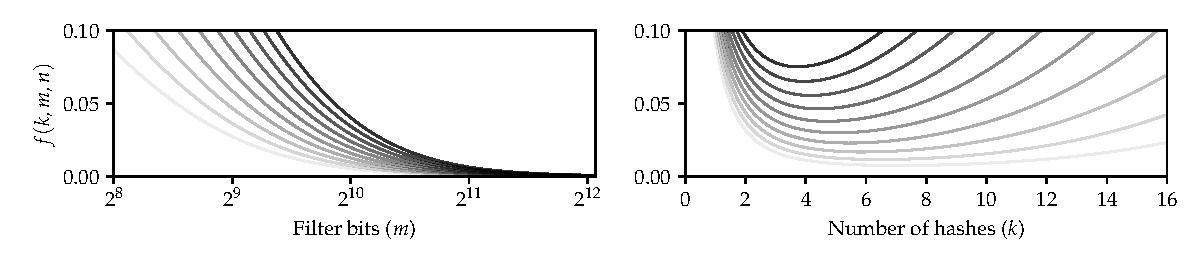
\includegraphics[page=1,scale=0.625]{fig/bf-viz}
  \vspace{-24pt}
  \caption{
    Function $f(k,m,n) = (1-e^{-kn/m})^k$ for various values of~$k$,
    $m$, and $n$.
    %
    In both plots, darker lines are for larger set sizes ($n$); values
    range from $n=100$ to~$200$.
    \textbf{Left:} varying filter length ($m$) and $k=4$ (the number
    of hash functions used in Squid).
    %
    \textbf{Right:} varying number of hashes ($k$) and $m=1024$.
    %
  }
  \vspace{6pt}
  \hrule
  \label{fig:bf-viz}
\end{figure}

This appendix summarizes the results of Kirsch and
Mitzenmacher~\cite{kirsch2006less} for the false-positive probability of Bloom
filters using double hashing.
%
Our presentation is less general than theirs, but suffices for understanding the
results in our paper.

\newcommand{\mset}{\procfont{mset}}
\newcommand{\hashscheme}{\capgreekfont{\Gamma}}
\heading{Additional notation.}
%
If~$\vv$ is a vector, then let~$\mset(\vv)$ denote the multiset comprised of its
elements.
%
Following~\cite{kirsch2006less}, if~$\setM$ is a multiset, we write $i,i
\in \setM$ to mean that~$i$ appears in~$\setM$ at least twice.

\heading{Hashing schemes.}
%
Let~$\elts$ be a set. A \emph{hashing scheme}~$\hashscheme$ for~$\elts$ is a
quadruple $(\hash, \length, \hashes, \sizes)$.
%
The last element is an infinite set $\sizes \subseteq \N$ denoting the permitted
\emph{set sizes}. (We do not require that $\sizes = \N$.)
%
Functions $\length$ and~$\hashes$ specify the filter length~$\length(n)$ and
number of hashes~$\hashes(n)$ respectively for set size~$n$.
%gq
The first element is a function~$\hash\colon\N\by\elts\to\N^*$ mapping a
parameter~$n\in\sizes$ and $x\in\elts$ to a $\hashes(n)$-vector of natural
numbers, which represent bit locations in a filter of length~$\length(n)$.
%
Formally, for every $n \in \sizes$, $\hash(n,\cdot)$ is a random function
specifying a joint distribution on a collection of random variables $\{
\hash(n,x)\colon x\in\elts\}$.
%
We associate to~$\hashscheme$, set~$\col\subseteq\elts$, and
$z\in\elts\setminus\col$ a \emph{false positive event}, denoted
$\FP(\col,z)$, which occurs if for every $j \in [\hashes(n)]$ there
exists some $x\in\col$ such that $\vv_j \in \mset(\hash(n,x))$, where $\vv =
\hash(n,z)$ and $n = \setlen{\col}$.

Fix a set~$\elts$ and a hashing scheme~$\hashscheme = (\hash, \length, \hashes,
\sizes)$ for~$\elts$.  Fix $z\in\elts$ and a collection of subsets $\{ \col_n
\}_{n\in\sizes}$ of $\elts$, where $z\not\in\col_n$ and $\setlen{\col_n} = n$
for each $n \in \sizes$.
%
The following says that, if~$\hashscheme$ satisfies certain conditions, the
false positive probability converges to the approximate bound
of~\cite{broder2004network} as~$n$ increases.
%
\begin{theorem}[Lemma 4.1 of~\cite{kirsch2006less}]
  \label{thm:mitz1}
  Suppose there exist $\lambda, k\in\N$ and a function $\gamma(n) \in o(1/n)$ such
  that for every $n \in \sizes$, it holds that
  \begin{enumerate}
    \item $\hashes(n) = k$;
    \item $\length(n) = O(n)$;
    \item $\{\hash(n, x)\colon x\in\elts\}$ are independent and
      identically distributed;

    \item for every $x \in \elts$, it holds that
      \[
        \max_{i\in\length(n)} \left|
          \Prob{ i \in \mset(\hash(n, x)) } - \lambda/kn
        \right| = O(\gamma(n)) \,;
      \]

    \item and for every $x \in \elts$, it holds that
      \[
        \max_{i,j\in\length(n)}
          \Prob{ i,j \in \mset(\hash(n, x)) } = O(\gamma(n)) \,.
      \]
  \end{enumerate}
  %
  Then $\lim_{n\goesto\infty} \Prob{\FP(\col_n,z)=1} = \left(1 -
  e^{-\lambda/k}\right)^k$.
\end{theorem}
%
Kirsch and Mitzenmacher prove that the \emph{double hashing scheme} defined by
\[
  \hash(n,x)_j = 1 + (h_1(n,x) + j\cdot h_2(n,x) \mod m(n)) \,,
\]
for each $j\in[k]$, where $k(n)=k$ and $m(n)=cn$ for some constants~$k$ and $c$, and
$h_1(n,\cdot)$ and~$h_2(n,\cdot)$ are independent and identically distributed
random functions with range $[m(n)]$, satisfies the conditions of
Theorem~\ref{thm:mitz1} for $\lambda = k^2/c$ and $\gamma(n) = 1/n^2$. (See
\cite[Thorem 5.2]{kirsch2006less}.) Thus, the false-positive probability
converges to $(1-e^{-k/c})^k$ as~$n\goesto\infty$.
%
But how close to this limit is the false positive probability for some
fixed~$n$? To address this question, Kirsch and Mitzenmacher provide an analysis
of the rate of convergence.
%
\begin{theorem}[Theorem 6.1 of~\cite{kirsch2006less}]\label{thm:mitz2}
  Suppose~$\hashscheme$ satisfies the conditions of Theorem~\ref{thm:mitz1}
  for~$\lambda$, $k$, and~$\gamma(n)$. For every~$n\in\sizes$, it holds that
  \[
    \left|
      \Prob{\FP(\col_n,z)=1} - \left(1 - e^{-\lambda/k}\right)^k
    \right| = O(n\gamma(n) + 1/n) \,.
  \]
\end{theorem}
%
For the double hashing scheme in particular, we have that the false positive
probability is at most
$
  (1 - e^{-k/c})^k + O(1/n)
$
for any $n\in\sizes$. (See~\cite[Theorem 6.2]{kirsch2006less}.)

Fix integers $k,m,n,\lambda \geq 0$ and let $H \colon \bits^* \to [m]^k$ and $F
\colon \bits^\lambda\by\bits^*\to[m]^k$ be functions.
%
Let $\struct_\saltybloom = \SBF[\hashbf[H],k,m,n,\lambda]$ and $\struct_\prfbloom =
\SKBF[\hashlin[F],k,m,n,\lambda]$ as defined in Figure~\ref{fig:bf-prf}.
%
If~$H$ and~$F$ are random functions, then $\hashbf[H]$ and $\hashlin[F]$ are
both realizations of the double hashing scheme for a particular choice of~$n$.
%
From Thoerem~\ref{thm:mitz2} it follows that the false positive probability
for~$\struct_\saltybloom$ and~$\struct_\prfbloom$ is at most
$
  (1 - e^{-kn/m})^k + O(1/n).
$
(See Figure~\ref{fig:bf-viz} for a visualization of this bound.)
%
In the proof of security for~$\struct_\saltybloom$
(Theorem~\ref{thm:bf-salt-correct}), we model~$H$ as a random oracle;
%
for~$\struct_\prfbloom$ (Theorem~\ref{thm:bf-prf-correct}), we can treat~$F$ as
a random function assuming it is a good PRF.


  \section{Proofs}
%  \input{appendix-proofs}
\end{appendix}

%\begin{thebibliography}{9}
%\bibitem{bloomfilter} 
%Burton Bloom.
%\textit{Space/time trade-offs in hash coding with allowable errors.}
%Commun. ACM 13, 7 (July 1970), 422-426.
%\end{thebibliography}

%\section{Old-stuff}
%\section{Tom's old Mutuable Hash-Based Filters}
Here we extend the basic Bloom filter syntax to allow for variations on the traditional Bloom filter, e.g. counting Bloom filters~\cite{xxx}, spectral Bloom filters~\cite{xxx}, count-min sketches~\cite{xxx}, stable Bloom filters~\cite{xxx}, etc.   Before giving it, let us briefly describe what is formalized.  Our syntax captures settings in which there is some (potentially empty) initial set~$S$, whose representation~$M$ may undergo updates over time.  Effectively, this allows for expansion of~$S$ to a larger set, or even a multiset, as new elements ``arrive''.    The update algorithm is responsible for altering the current representation.  We allow it to take in a string that encodes inputs needed to carry out the updating.  For example, counting Bloom filters may receive update strings that encode $(x,c)$ where $x \in U$ is the element whose representation should be incremented, and $c \in \mathbb{N}$ is the amount of the increment.  Network applications, such as looking for heavy-hitters across TCP/IP streams seen by a router, may have $x = (\mathrm{IP_{src}},\mathrm{IP_{dst}})$, the source and destintation address of a packet, and~$c$ the number of bytes in the packet payload.  When necessary we will specify what is encoded in the update string, but will assume some implicit and fixed encoding scheme.  Note that our syntax allows for randomized updating.  This accommodates stable Bloom filters, for example, which has a randomized ``forgetting'' feature as part of its update.

\heading{Preliminaries.}
When~$U$ is a set, we let $\multiset{U}{}$ denote the set of all finite multisets of~$U$.  We can denote any multiset~$S$ as $\{(x,\ell) \,|\, x \in U, \ell > 0\}$ where each~$x$ appears exactly once, and each~$\ell$ is an integer.  We define the multiplicity of~$x$ as $\mu_S(x) = \ell$.  We write $|S|= \sum_{(x,\ell)\in S}\mu_S(x)$, and let $\multiset{U}{n}$ denote the set of multisets~$S$ where $|S|=n$.   The notation $S \uplus \{x\}$ denotes multiset union.

\heading{Syntax. }
Fix nonempty sets $U,\Sigma$ and integers $k,m_1,m_2,n>0$ with $m_1 \leq m_2$.  Fix a symbol $\bot \not\in U$.  An $(n,k,[m_1,m_2])$-filter (over universe~$U$) is a tuple  $B=(\Hash,\Init,\Qry,\Update, \Test)$.   
%
The randomized \emph{hash-sampling} algorithm~$\Hash$ samples a size~$k$ family of functions~$\mathcal{H}=\{h_1,h_2,\ldots,h_k\}$ where each $h_i \in  \mathrm{Func}(U,\{0,1,\ldots,m_2-1\})$.  We write $\mathcal{H} \getsr \Hash$ for this operation. 
%
The randomized \emph{initial-representation} algorithm $\Init\colon \multiset{U}{n} \rightarrow \left(\bigcup_{m=m_1}^{m_2}\Sigma^m\right) \times \bits^*$ takes a multiset~$S$ of size~$n$ as input, and outputs representation~$M$ of length~$m_1 \leq m \leq m_2$, and side-information~$\tau$.
%
The determinisitc query algorithm $\Qry\colon \left(\bigcup_{m=m_1}^{m_2}\Sigma^m \right)\times \bits^* \times U \rightarrow \bits^*$ takes a representation $M$, side-information~$\tau$, and an element $x \in U$ as input, and returns a bitstring.  
%
The randomized \emph{update} algorithm $\Update\colon \left(\bigcup_{m=m_1}^{m_2}\Sigma^m \right)\times \bits^* \times \bits^*\rightarrow \left(\bigcup_{m=m_1}^{m_2}\Sigma^m \right) \cup \{\bot\}$ takes a representation~$M$, side-information~$\tau$, and an update string~$\sigma$ as input, and returns an updated representation or the distinguished symbol~$\bot$.  
%
The deterministic \emph{test} algorithm $\Test \colon \multiset{U}{} \times \left(\bigcup_{m=m_1}^{m_2}\Sigma^m \right)\cup\{\bot\} \times \bits^* \times U \rightarrow \bits$ takes a multiset~$S$, a representation~$M$, side-information~$\tau$, and an element~$x \in U$ as input, and returns a bit. \tsnote{The point of $\Test$ is to capture correctness, which is not guaranteed in this setting.  (It isn't something one would actually implement in practice.)  Intuitively, $\Test$ outputs 1 iff $x \in S$ but the representation~$M$ ``says'' it is not.}
%
%We assume that all $\Init,\Qry,\Update,\Test$ all have blackbox access to the functions $h_1,h_2,\ldots,h_k \in \mathcal{H}$, which we denote by writing~$\mathcal{H}$ as a superscript.   

\heading{Correctness. } The kind of filters we capture, here, can have \emph{two-sided} error.  That is, they may result in false-negatives as well as false-positives.  We captures two versions of correctness in Figure~\ref{fig:correctness-mutable}, corresponding to whether or not the adversary is given access to the hash functions used to create and update the multiset representation. \tsnote{These are draft experiments!}

\begin{figure}
\centering
\fpage{.75}{
\hpagess{.6}{.35}
{
\experimentv{$\ExpCorrectSecHash{B}{\distr{U}{n}, A}$}\\
$S \getsr \distr{U}{n}$\\
$ \{h_1,h_2,\ldots,h_k\} \getsr \Hash$\\
$(M,\tau) \getsr \Init^{\HashOracle}(S)$\\
$x \getsr A^{\QryOracle,\UpdateOracle}(S)$\\
if $\Test^{\HashOracle}(S,M,\tau,x) \neq 1$ then\\
\nudge Ret 1\\
Ret 0
}
%
{
\oracle{$\QryOracle(x)$}\\
if $M = \bot$ then Ret $\bot$\\
Ret $\Qry^{\HashOracle}(M,\tau,x)$\\

\medskip
\oracle{$\UpdateOracle(\sigma)$}\\
if $M = \bot$ then Ret $\bot$ \\
$\mathrm{op},\mathrm{val} \gets \sigma$\\
$S \gets S \uplus \{\mathrm{val}\}$\\
$M \getsr \Update^{\HashOracle}(M,\tau,\sigma)$\\

\medskip
\oracle{$\HashOracle(i,x)$}\\
Ret $h_i(x)$\\
}
}
%%%%%%%%%%
\fpage{.75}{
\hpagess{.6}{.35}
{
\experimentv{$\ExpCorrectPubHashBB{B}{\distr{U}{n} , A}$}\\
$S \getsr \distr{U}{n}$\\
$ \{h_1,h_2,\ldots,h_k\} \getsr \Hash$\\
$(M,\tau) \getsr \Init^{\HashOracle}(S)$\\
$x \getsr A^{\QryOracle,\UpdateOracle,\HashOracle}(S)$\\
if $\Test^{\HashOracle}(S,M,\tau,x) \neq 1$ then Ret 1\\
Ret 0
}
%
{
\oracle{$\QryOracle(x)$}\\
if $M = \bot$ then Ret $\bot$\\
Ret $\Qry^{\HashOracle}(M,\tau,x)$\\

\medskip
\oracle{$\UpdateOracle(\sigma)$}\\
if $M = \bot$ then Ret $\bot$ \\
$\mathrm{op},\mathrm{val} \gets \sigma$\\
$S \gets S \uplus \{\mathrm{val}\}$\\
$M \getsr \Update^{\HashOracle}(M,\tau,\sigma)$\\

\medskip
\oracle{$\HashOracle(i,x)$}\\
Ret $h_i(x)$\\
}
}
%%%%%%%%%%%
\fpage{.75}{
\hpagess{.6}{.35}
{
\experimentv{$\ExpCorrectPubHash{B}{\distr{U}{n} , A}$}\\
$S \getsr \distr{U}{n}$\\
$ \{h_1,h_2,\ldots,h_k\} \getsr \Hash$\\
$(M,\tau) \getsr \Init^{\HashOracle}(S)$\\
$x \getsr A^{\QryOracle,\UpdateOracle}(S,\{h_1,h_2,\ldots,h_k\})$\\
if $\Test^{\HashOracle}(S,M,\tau,x) \neq 1$ then Ret 1\\
Ret 0
}
%
{
\oracle{$\QryOracle(x)$}\\
if $M = \bot$ then Ret $\bot$\\
Ret $\Qry^{\HashOracle}(M,\tau,x)$\\

\medskip
\oracle{$\UpdateOracle(\sigma)$}\\
if $M = \bot$ then Ret $\bot$ \\
$\mathrm{op},\mathrm{val} \gets \sigma$\\
$S \gets S \uplus \{\\mathrm{val}\}$\\
$M \getsr \Update^{\HashOracle}(M,\tau,\sigma)$\\

\medskip
\oracle{$\HashOracle(i,x)$}\\
Ret $h_i(x)$\\
}
}
\caption{Trying to define correctness for an $(n,k,[m_1,m_2])$-filter~$B$.  \textcolor{cyan}{Revisit once picture for ``plain'' filters settles.  Also, not exactly right since $\distr{U}{n}$ currently defined to sample from $[U]^n$; here should be multisets.}}
\label{fig:correctness-mutable}
\end{figure}


\heading{Soundness for mutable hash-based filters. } \tsnote{To do.  Same comments as for the simple case, only it's more complicated here because I have no idea what soundness even means in this setting.  Might generically specify two tests as part of the syntax, one for correctness and one for soundness?}


\heading{Privacy of Mutable hash-based filters.} \tsnote{To-do.}


%%%%%%%%%%%%%%%%%%%%%%%%%%%%%%%%%%%%%%%%%%%%%%%%%%%%%%%%%%%%%%%%%
\section{Security Results for Mutable Hash-Based Filters}
\begin{itemize}
\item Prove privacy of ``Stable'' Bloom Filters
\item Ditto for count-min sketch (with and without conservative update)
\item Ditto for scaling BF 
\item Correctness and soundness bounds for these?  (Not sure this is possible without a lot of work; see what's already been done in the papers that propose them)
\end{itemize}

%%%%%%%%%%%%%%%%%%%%%%%%%%%%%%%%%%%%%%%%%%%%%%%%%%%%%%%%%%%%%%%%%

\if{0}
\heading{Multiset-oriented hash-based filters. }
\tsnote{Commented out, but in the source: an alternative way to formalize mutable hash-based filters.  This way directly address the inputs as multisets, instead of starting with a set and then updating the represenation a step at a time.  Not sure which is cleaner and more easily applied to real problems, yet.}

Let $\mathbb{M}_\mathcal{U}$ be the set of multisets over~$\mathcal{U}$.  We can denote any multiset as $\{(x,\ell) \,|\, x \in \mathcal{U}, \ell \in \mathbb{N}\}$, and for a particular multiset~$S$ we define the multiplicity of~$x$ as $\mu_S(x) = \ell$ where $(x,\ell)\in S$.

An $(n,k,[m_1,m_2])$-filter with operations is a tuple  $B=(\Hash,\Rep,\Qry, \mathcal{F})$.  
The set $\mathcal{F}$ is the finite collection of allowable operations.  All operations are of the form 
$f: \mathbb{M}_{\mathcal{U}} \times \mathbb{M}_{\mathcal{U}} \rightarrow \mathbb{M}_{\mathcal{U}} \cup \{\bot\}$.  
%
The deterministic representation algorithm $\Rep\colon \mathbb{M}_\mathcal{U} \rightarrow \bigcup_{m=m_1}^{m_2}\Sigma^m$ takes a multiset~$S$, and outputs representation~$M$ of length~$m_1 \leq m \leq m_2$, or the distinguished symbol~$\bot$.  We assume that if the multiset~$S=\{(x_1,\ell_1),(x_2,\ell_2),\ldots,(x_t,\ell_t)\}$ is such that $n < \sum_{i=1}^t \ell_i$ then $\Rep(S)=\bot$.
%
The randomized hash-sampling algorithm~$\Hash$ is as before.
%
The determinisitic query algorithm $\Qry$... \tsnote{Not sure how to define this!  See my comment, below...}

%Correctness is defined as follows.  Let $S,T$ be arbitrary multisets and let~$f$ be an arbitrary operation in $\mathcal{F}$.  If $f(S,T) = S'\neq \bot$, then for all $x \in S'$ we demand that $\Qry(\Rep(S'),x)=1$.  \tsnote{might need a stronger condition that this holds for any sequence of operations that do not result in $\bot$.}

Let us see how this syntax captures various kinds of Bloom filters.  First, let $\Sigma = \mathbb{N}$ and define $f_{\mathrm{add}}(S,T)=\{(x,\mu_S(x)+\mu_T(x)) \,|\, x \in \mathcal{U}\}$ and $f_\mathrm{del}(S,T) = \{(x,\min\{0,\mu_S(x)-\mu_T(x)\}) \,|\, x \in \mathcal{U} \}$.  Define $\Rep(S')$ as follows: for each $(x,\ell)\in S'$ and $j\in\{1,2,\ldots,k\}$, set $M[h_j(x)]=\ell$.   Finally, define $\Qry(M,x) = 1 \Leftrightarrow \forall j \in \{1,2,\ldots,k\},\; M[h_j(x)] > 0$.  This allows us to capture counting Bloom filters. \tsnote{Does it?  Acutally, you might want $\Qry(M,x)$ to return a number, i.e., a counter value.  How do you define correctness then?}

\tsnote{There are more direct ways to formalize counting Bloom filters, like the syntax above.  But this less direct way will allow us to capture other kinds ``advanced'' Bloom filters proposed in the literature or (more importantly) used in practice. For example, $f_{\mathrm{setify}}(S,T)=\{(x,1) \,|\, x \in \mathcal{U} \mbox{s.t. } \mu_S(x)>0, \mu_T(x)>0\}$.  On the other hand, we may end up deciding it is overkill... }
\fi


\end{document}